%% Digital Discovery manuscript (revision after mock review).
%% Layout approximates the RSC two-column article template; paste the body into
%% the official RSC template before submission.
\documentclass[twocolumn,10pt]{article}
\usepackage[a4paper,margin=1.7cm,columnsep=0.6cm]{geometry}
\usepackage{mathptmx}
\usepackage[T1]{fontenc}
\usepackage{amsmath,amssymb}
\usepackage{graphicx}
\usepackage{booktabs}
\usepackage[super,sort&compress,comma]{natbib}
\usepackage[font=small,labelfont=bf]{caption}
\usepackage{xcolor}
\usepackage{xr-hyper}
\usepackage[hidelinks]{hyperref}
\externaldocument[esi-]{esi}
\makeatletter\newcommand{\inputrows}[1]{\@@input #1 }\makeatother
\newcommand{\todo}[1]{\textcolor{red}{[#1]}}
\newcommand{\placeholder}[2]{\fbox{\parbox[c][#1][c]{0.95\linewidth}{\centering\small\textcolor{red}{#2}}}}
\setlength{\parskip}{0pt}
\raggedbottom

\title{\Large\bfseries Audit the chemistry you will screen:\\ count-level guarantees for a screening round}
\author{Petrus H. Zwart\thanks{Center for Advanced Mathematics in Energy Research Applications, Berkeley Synchrotron Infrared Structural Biology Program, and Molecular Biophysics and Integrated Bioimaging Division, Lawrence Berkeley National Laboratory, 1 Cyclotron Road, Berkeley, CA 94720, USA. E-mail: PHZwart@lbl.gov. Electronic supplementary information (ESI) available: derivations, algorithms, simulation protocols and additional tables.}}
\date{}

\begin{document}
\twocolumn[
\maketitle
\begin{abstract}
Conformal prediction supplies prediction sets with guaranteed coverage, and is increasingly
applied to screening in chemistry and materials science. A screening round, however, is planned
in counts rather than rates. A laboratory commits wells on a plate, the reagent budget of a run,
and the hits it must confirm to justify going on. Forecasting such counts for a batch not yet
assembled takes a labelled audit set. That sample must come from the library the round will draw
on, and serve neither training nor calibration. The exchangeability it needs differs
from the one underpinning coverage. Seen from the audit, a calibration set is training data.
Coverage and the predicted counts therefore become separate guarantees, and their asymmetry runs
in a single direction. A classifier tuned on the wrong population, prevalence or label predicts
less well, although auditing it stays sound. An audit sampling chemistry the batch lacks voids
the forecast, however carefully that tuning was done. We examine four arrangements in which this
second requirement fails on public data. Withholding building blocks in a DNA-encoded library
cost two thirds of the coverage, while the ranking slipped from 0.960 to 0.892 in area under the
curve, roughly a seventh of its margin above chance. Where the model itself chose the batch, no
audit could be reserved from the library in nine of twelve rounds. None of the figures a screen
ordinarily reports ranks these failures. Two designs held. One is a pilot of the population to be
screened. The other is a random slice of the committed round, which remains exact whatever rule
selected it.
\end{abstract}
\vspace{1em}
]

%% ------------------------------------------------------------------
\section{Introduction}
\label{sec:intro}

Anticipating how a model behaves on data it has not seen is central to the machine learning now
applied to chemical and materials screening. Two divisions of a dataset are commonly made. The
training compounds are first held apart by scaffold or by building block, which tests whether a
model has memorised the chemistry it was shown, and a ranking surviving that test is read as
evidence of transfer. What remains is then split at random to calibrate a decision rule, which
fixes the error rates that rule will realize. Both steps are routine. The warrants they confer,
however, are different, and neither extends to the other's.

The two are easily confused, and the price of that runs in opposite directions. A structural
holdout does establish that a ranking transfers to new chemistry. It also invalidates every
quantitative statement about the next batch. Withholding building blocks in a
DNA-encoded library cost two thirds of the coverage of the predicted counts, while the ranking
slipped from 0.960 to 0.892 in area under the curve, roughly a seventh of its margin above
chance. A random division keeps those counts sound, although only for whatever it sampled, which
is seldom what a round commits. Where a planner fills a plate from the head of a scored
list, an audit held back from the library will not price it. In nine of twelve rounds of the
campaign described below no such audit could be built, since no in-class candidate was left in
the remaining pool to measure. One step therefore secures a quantity no round is planned on. The
other bounds the right quantities for the wrong population, and this paper is about what a
labelled sample does and does not license a team to claim.

Such claims must be stated in counts. A round is constrained in integers, by the wells on a
plate, the reagent budget of a run, and the confirmed hits needed before a further round can be
justified. Those constraints do not translate into rates. An error rate that is slightly
optimistic will go unnoticed, whereas a plate exceeding its capacity halts the experiment.
Conformal prediction wraps any trained model and returns prediction sets whose coverage is
guaranteed under
exchangeability.\citep{vovk2005algorithmic,AngelopoulosBates2023Gentle} It does not,
however, yield counts. Coverage is a level the user selects and the threshold is built to meet,
so every setting is equally guaranteed and coverage ranks none of them. Risk-controlling methods
bound a chosen loss, although what they control is its expectation, or the probability of
exceeding it,\citep{bates2021distribution,Angelopoulos2024CRC,Angelopoulos2021LTT} rather than the
integer a run returns. The post hoc literature does bound counts, though for a set already in hand; the batch in question has yet to be assembled. What a campaign lacks is a \emph{predictive} count,
meaning a statement about a batch not yet made. A labelled audit set supplies one, and how that
sample is drawn is the subject of this paper.

The screens we consider decide which candidates go forward to a toxicity assay, a solubility or
conductivity measurement, or synthesis. Because characterization runs in parallel, a round's
capacity is fixed before it begins. Unlike turn-by-turn optimization, a batch campaign often aims at covering a design space
(Section~\ref{sec:discussion}). In a binary screen each compound receives one of four prediction
sets, holding one label, the other, both, or neither. A team advances or discards the compounds
given a single label and sends the rest for assay. Before committing it needs to know how many
will fall into each case.

\paragraph{What we do.} We treat the coverage level as a control rather than a result. It is
chosen separately for the in-class and out-class compounds, and sweeping it moves the classifier
through the space of available rounds. A labelled \emph{audit set}, sampled from the library to
be screened and used for neither training nor calibration, then prices each setting. It gives
the confident hits, false leads, missed in-class compounds and assays that a batch of the
committed size will contain, each as a count with a finite-sample interval valid under
exchangeability of the audit with the batch. These intervals are the deliverable, against which
assays can be booked and measurements budgeted. The condition they require differs from the one
coverage assumes, and Section~\ref{sec:methods:intervals} separates the two.

In the remainder of this paper we set out the outcome table, the threshold correction and the
audit intervals that the method returns, together with the role coverage plays in navigating
them. We then validate those intervals in simulation and on measured data, and apply them to
solubility, toxicity and electrolyte screens. A workflow and the limitations close the paper.

\paragraph{Contributions.} The statistical tools are classical; what is new is the separation
they make visible and what violating it costs.

\begin{itemize}\itemsep2pt
\item \emph{A labelled audit set prices a round, in counts, before it is run.} Sweeping the two
class-wise coverage requests traces the decisions available to a team, and at each setting an
audit gives finite-sample intervals for every cell of the outcome table, covering confident hits, false leads, missed in-class compounds and compounds assayed, valid after the setting is chosen
and invertible for the size of the round.\citep{Thatcher1964,Meeker2017Intervals}
\item \emph{Two guarantees, two requirements, and the asymmetry runs one way.} From the audit's
point of view the calibration set is training data, so coverage and predicted counts fail
independently (Table~\ref{tab:decoupling}); a rule calibrated on the wrong population,
prevalence or label is a worse rule but a valid audit, while an audit drawn from chemistry the
batch does not share voids the counts however the rule was calibrated.
\item \emph{What violating it costs, measured four ways on real data.} Withheld building blocks,
division by provenance, an audit matching a batch's composition but not its chemistry, and a
batch the model chose: the counts break in all four, and no statistic a screen reports orders
the failures.
\item \emph{What satisfying it takes.} A pilot of the screened population repairs it under
divisions that are not random, and a random slice of a committed batch repairs it exactly,
whatever rule selected the batch. One round of selection then depletes the library, so the slice is re-drawn each round.
\item \emph{A check that costs no measurements.} Whether the audit matches the batch is testable
beforehand from structures alone, as a classifier two-sample test against a permutation
null.\citep{LopezPaz2017Revisiting} The test is one-sided, so it can refuse an arrangement but never certify one, and is blind by construction to a shift the representation cannot see.
\end{itemize}

\paragraph{Related work.}
\label{sec:intro:related}
Conformal prediction is established in cheminformatics, for toxicity, bioactivity, imbalanced data, applicability domain and drift.\citep{Norinder2014,NorinderBoyer2017,Sun2017Mondrian,Svensson2017,Bosc2019,CortesCiriano2019,Morger2021,Geylan2024,CPSign2024,Laghuvarapu2023CoDrug} The closest work estimates what a screening round will return. Buendia \textit{et al.}\ predict the number of hits an iteration of an iterative high-throughput screen will retrieve, by summing per-compound calibrated probabilities from Venn--ABERS predictors over the selected compounds, and show across six targets that the sum tracks the realized count;\citep{Buendia2019Hit,Buendia2018VAP} Svensson \textit{et al.}\ link conformal predictions to the gain of a screen.\citep{Svensson2018Gain} Estimating campaign-level counts is therefore established, and we build on it. A sum of calibrated probabilities is an expectation, and we add a probability statement about the realized count, which is what a plan that has to hold requires. Buendia \textit{et al.}\ also identify the obstacle to such a statement: selecting the highest-ranked compounds leaves the calibration and screened sets progressively less exchangeable, retaining validity would require measuring a fresh random subset of the screened library at every iteration, and the cost of those measurements would make the approach impractical. They therefore keep the initial calibration set, and report that the realized hit count falls outside their expected limits in later iterations. That randomly chosen, measured subset is the audit set used here, and its cost can be set against the compounds it saves (Section~\ref{sec:results:sizing}). These studies report coverage and efficiency, or a gain, on test data; we add prediction intervals for what a future batch will contain. In statistics, the coverage of a conformal predictor given its calibration set is known exactly,\citep{Vovk2012PAC,Bian2023TrainingConditional,Marques2025Beta} and related to tolerance regions and PAC prediction sets.\citep{Wilks1941,Park2020PAC} Risk-controlling methods are the closest prior art and the comparison is worth making
precisely, because they answer a different question altogether. Conformal risk control bounds an expectation, $\mathbb{E}[L_{n+1}(\hat\lambda)]\le\alpha$,
marginally over the calibration set and the test point together, for a single future point, under a loss required
to be monotone in a scalar parameter.\citep{Angelopoulos2024CRC} The decisive restriction concerns what the loss is defined on, and not what it measures: $L_{n+1}$ is a loss at a single future point, and a
constraint such as ``this plate of $m$ did not overrun its capacity'' is a functional of the
whole batch, which is not of that form. Risk-controlling prediction sets make the statement
high-probability and conditional on the calibration set,
$\Pr(R(\hat\lambda)\le\alpha)\ge1-\delta$,\citep{bates2021distribution} and learn-then-test
reaches batch-level functionals, controlling any risk that admits a concentration bound over
several parameters and constraints at once.\citep{Angelopoulos2021LTT} What that route needs is
a sample of the thing it controls: to bound the risk of a round empirically, one needs rounds.
A campaign has one, and it is the round being priced. The construction below takes its
probability from inside that single round, by conditioning on the audit-and-batch total, which
is how it can speak about a batch of $m$ before the batch exists. Two lines of work do bound counts in a batch
not yet measured, and both are nearer to this paper than the rate-control family. Gazin
\textit{et al.}\ show that the $m$ conformal $p$-values of an \emph{unlabelled} test batch
follow a P\'olya urn law, and give a concentration inequality for their empirical distribution
function;\citep{Gazin2024Transductive} scaled by $m$, that bounds how many of the batch fall
below a threshold, with no measurement on the batch at all. The exchangeability combinatorics
are the same ones the construction below runs twice, and we claim no priority over them. Song
\textit{et al.}\ bound the false discovery proportion of a conformal selection simultaneously
over all thresholds, so that a threshold may be chosen after the data are
seen;\citep{Song2026FDP} since the selected set is observed once the batch has been scored,
that envelope multiplied by its size is likewise a high-probability bound on an integer in an
unmeasured batch, and a sharper instrument than the Bonferroni correction we use for the same
purpose.

What a labelled audit buys is therefore a particular quantity under a particular condition, since counting and predicting are both already available. Those bounds are one-sided, bounding false
discoveries without placing a floor under yield. They are statements about the selected set, so
they are silent on every cell an \emph{unselected} in-class compound defines, since a missed hit does not appear in the selection. They do not invert for the batch size. And, most consequentially here,
what they require is exchangeability between calibration and test, which is precisely the
condition a structural split breaks; the intervals below require exchangeability between audit
and batch, a different condition that holds and fails in different circumstances
(Table~\ref{tab:decoupling}). The price of the second is measurement.

Bounding a realized count in a finite selected set is older than any of this and is not ours.
Confidence envelopes for the false discovery proportion go back to Genovese and
Wasserman,\citep{GenoveseWasserman2004} and the post hoc, true-discovery literature gives
simultaneous high-probability bounds on the number of true discoveries in an arbitrary selected
set, with closed-testing shortcuts that make them
computable.\citep{Goeman2011Exploratory,Goeman2019Simultaneous,Katsevich2020FDP,Blanchard2020PostHoc}
These are two-sided in the operational sense: an envelope on the false discovery proportion
gives a capacity ceiling and a lower confidence bound on true discoveries gives a yield floor.
Neither is label-free. Each needs a $p$-value for every unit of the set it bounds, that
is one measurement per unit, which is a higher price than an audit's and not a lower one, since
the audit measures a sample and then speaks about units it never measured. The direction they
cannot reach is the one a planner needs. Closed testing bounds a non-null proportion from
below, so taking the discarded set as the selection gives a lower confidence bound on the hits
thrown away but not an upper one, and it is the upper limit on misses that tells a team whether
a setting is safe to commit.

A campaign is constrained in counts, not rates, and the two differ by more than a rounding. A
guarantee that the long-run failure rate is at most 0.1 does not say that a plate of 96 will
hold at most 13 failures with probability 0.95, because the realized count varies around the
rate by an amount the rate bound does not describe. That variability is not a correction at the
scale these platforms run: at an audit of 400 and a batch of 50, 89\% of the variance of the
interval reported here is contributed by the draw of the batch rather than by uncertainty in the
rate (Section~\ref{sec:results:sizing}). A bound on the rate alone therefore leaves the
larger part of that variability undescribed, and leaves most of it undescribed exactly where
autonomous platforms operate, in small batches run often. A rate bound can of course be composed with a
binomial tail to yield a count bound, and the composition is valid. It pays twice, once for the
rate and once for the tail, where conditioning on the audit-and-batch total pays once, and the
price is measurable. Giving the rate bound the most generous instrument available, an exact Clopper--Pearson limit in place of the concentration bounds risk-controlling sets actually use, and splitting the level evenly between its two stages, which is what makes the composition
valid at a one-sided 0.05 overall, the composed limit sits 11 to 60\% above the exact inversion
over the configurations this paper reports. Measured as a planner would, in the headroom that
has to be reserved above the expected count, the gap is larger: pricing one plate of 96 from an
audit of 384 at a 2\% rate, the exact bound allows 5 confident hits and the composition 8, so
the headroom doubles, from three compounds above the expected two to six
(ESI Section~\ref{esi-sec:compose}). The composition also assumes more. Its second stage treats the batch count as binomial given the
rate, which holds when the batch is an independent sample from a fixed distribution but not for
a finite exchangeable sequence, which need not be a mixture of independent
ones;\citep{DiaconisFreedman1980} the hypergeometric argument needs no such representation
(ESI Section~\ref{esi-sec:target}). The construction here bounds the realized integer count in
a batch of stated size, two-sided so that capacity and yield can both be constrained, for every
cell of the outcome table rather than one monotone summary, without any monotonicity
requirement, and invertible for the batch size itself. Prediction-powered inference gives distribution-free intervals for an aggregate functional
from a small gold-standard sample together with a model's predictions on the
rest,\citep{Angelopoulos2023PPI} which is the audit set's role for the rate term; what it does
not supply is the second term, the variation of a realized count about that rate in a batch of
the committed size. Conformal selection\citep{JinCandes2023} selects candidates with false-discovery control, and set-valued classifiers with bounded class-wise error\citep{Sadinle2019} minimize ambiguity. Decision-theoretic work links prediction sets to actions. Conformal decision theory calibrates a decision parameter to a target risk,\citep{Lekeufack2024CDT} and Kiyani \textit{et al.}\ showed that prediction sets are a sufficient statistic for risk-averse decision makers with a known utility, for whom acting on the worst case within the set is optimal.\citep{Kiyani2025RAC} The question for which costs a classifier, or an abstaining classifier, is optimal goes back to the reject option\citep{Chow1970} and to ROC analysis.\citep{ProvostFawcett2001,Pietraszek2005} Our aim is complementary. We assume no utility, report \emph{all} screening outcomes of each coverage setting with valid intervals and bounds, and let a team choose afterwards under its own objective and constraints.

%% ------------------------------------------------------------------
\section{Methods}
\label{sec:methods}

\subsection{Setting and assumptions}
\label{sec:methods:setting}

We call the class with the property the screen looks for \emph{in-class} (label 1) and the other \emph{out-class} (label 0): compounds active at an endpoint in Tox21, soluble compounds in AqSolDB, and electrolytes that reach the conductivity target in CALiSol-23. A trained binary classifier is held fixed. It gives each compound a predicted probability of being in-class, $u=\hat p(\text{in-class}\mid x)$. A labelled \emph{calibration set} sets the thresholds. A labelled \emph{audit set}, which in machine-learning terms is a held-out test set, is used only to measure what the thresholds do; we call it an audit set throughout, because its purpose here is to price a round. A \emph{future batch} of $m$ compounds will be screened. We assume throughout that the audit and future compounds are exchangeable with one another given the trained model and the calibration set, \textit{i.e.}\ that their joint distribution is unchanged when they are reordered. The requirement is conditional on the calibration set, which need not itself be exchangeable with either; a random division of a fixed library satisfies it even though the three parts are then dependent through the library's finite size. Where the coverage guarantee is also wanted, the calibration set must in addition be exchangeable with the batch; the two requirements are separated in Section~\ref{sec:methods:intervals} and they fail independently. What must be exchangeable is each candidate together with the label recorded for it, not the candidate alone, so the assumption can fail in two ways that look nothing alike: the compounds may be drawn from different populations, or the compounds may be interchangeable while the label recorded on one set is not the label recorded on another. The first is a question of which compounds a round contains and the second of what is measured on them, and both appear below. Exchangeability holds when all three sets are random samples of the library to be screened and carry the same label. The training set is deliberately absent from that list. The classifier is held fixed and enters only as a score, so how its training compounds were chosen bears on how good that score is and not on whether the intervals are valid. The two splits a campaign makes are therefore independent and answer different questions. Separating the training compounds from the rest by scaffold, series or building block guards against a model that has memorised its training chemistry, and lowers an optimistic estimate of how well it ranks compounds unlike the ones it was fitted on. Dividing what remains into calibration, audit and batch at random is what keeps the intervals valid. Both can be done at once, and should be: the arrangement that measures a model on unseen chemistry \emph{and} prices the batch correctly is a split at the training boundary followed by random assignment within the deployment population. The unit of sampling is the candidate to be screened: a compound, or for electrolytes a formulation, and not an individual measurement. It fails when the batch comes from other chemical series or scaffolds (Section~\ref{sec:results:dependence}), and again when the thresholds are set against a cheaper label than the one the campaign's claim concerns (Section~\ref{sec:results:surrogate}). It fails too when the batch is chosen using the model, as in active learning, unless that selection is part of the design. Section~\ref{sec:results:adaptive} tests that case and the two repairs available for it. The probabilities need not be calibrated in the usual sense; only their ordering matters.

\subsection{Prediction sets and the outcome table}
\label{sec:methods:table}

We use class-conditional (Mondrian) split conformal prediction,\citep{vovk2005algorithmic} which controls coverage separately for the in-class and out-class compounds. The label \emph{out-class} is included in a compound's prediction set when $u\le\tau_0$, where $\tau_0$ is set from the out-class calibration compounds. The label \emph{in-class} is included when $u\ge1-\tau_1$, where $\tau_1$ is set from the in-class calibration compounds (Fig.~\ref{fig:sets}; ESI Section~\ref{esi-sec:notation}). Each compound then falls into one cell of a $2\times4$ table of true label by prediction set (Table~\ref{tab:outcomes}). Every screening quantity is a sum of cells:
\begin{itemize}
\item missed in-class compounds are in-class compounds labelled $\{\text{out-class}\}$;
\item false leads are out-class compounds labelled $\{\text{in-class}\}$, \textit{i.e.}\ compounds followed up that turn out out-class;
\item deferred compounds receive both labels or none;
\item coverage is the sum of the cells in which the true label is in the set;
\item the hit rate of the confident calls is a ratio of two cells.
\end{itemize}
The cells in each row add up to the number of compounds of that class. Moving a threshold therefore moves compounds between cells of the same row, so the outcomes trade off against each other. With class probabilities, a compound can receive both labels or none, but not both kinds for the same thresholds (ESI Section~\ref{esi-sec:geometry}). We report the two kinds separately, because an empty set signals a compound unlike the calibration data and not merely an ambiguous one.\citep{Norinder2014}

\begin{figure}[t]
\centering
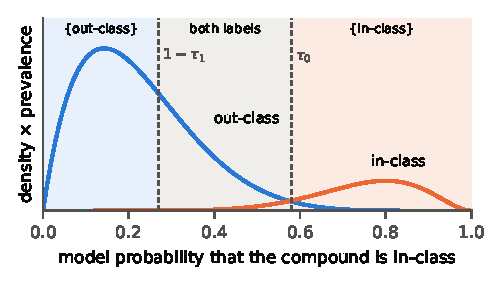
\includegraphics[width=\columnwidth]{figures/fig1_prediction_sets.pdf}
\caption{Class-conditional thresholds divide compounds into prediction sets. Curves show the distribution of the predicted probability of being in-class for out-class (blue) and in-class (orange) compounds, weighted by prevalence. Compounds left of $1-\tau_1$ receive $\{\text{out-class}\}$, those right of $\tau_0$ receive $\{\text{in-class}\}$, and those in between receive both labels. If the thresholds cross, the middle band receives the empty set instead. The coverage request for each class moves one threshold.}
\label{fig:sets}
\end{figure}

\begin{table}[t]
\centering
\caption{Outcomes of a binary conformal screen. Each compound falls into one cell; every screening quantity is a sum of cells.}
\label{tab:outcomes}
\small
\begin{tabular}{@{}lcccc@{}}
\toprule
True label & $\{\text{out-class}\}$ & $\{\text{in-class}\}$ & both & none \\
\midrule
out-class & correct rejection & false lead & deferred & deferred \\
in-class   & missed in-class & confident hit & deferred & deferred \\
\bottomrule
\end{tabular}
\end{table}

\subsection{Coverage requests and thresholds}
\label{sec:methods:thresholds}

The standard threshold guarantees coverage of at least $1-\alpha$ only on average over calibration sets. With tens of in-class calibration compounds, the coverage of the one model actually deployed can fall well below $1-\alpha$. The coverage observed over a batch of $m_y$ future compounds of class $y$ follows a Beta--Binomial distribution that depends only on the number of calibration compounds of that class and on the chosen order statistic. This result requires only exchangeability. It is the classical distribution-free rank law behind Wilks--Wald tolerance limits, read in the conformal setting;\citep{Wilks1941,Vovk2012PAC,Marques2025Beta} the correction rule built from it is a two-parameter tolerance limit transposed to a finite batch. We choose the least conservative threshold for which batch coverage is at least $1-\alpha_y$ with probability at least $1-\delta_y$, separately for each class. A coverage request therefore has four numbers, $(\alpha_0,\delta_0,\alpha_1,\delta_1)$. The guarantee is stated for a planned number $m_y$ of future compounds of each class, which we set from the batch size and the class proportions of the calibration set. That is a plug-in for a quantity the campaign does not know, and at low prevalence it is estimated from few compounds, so the tolerance $\delta$ is controlled for the planned count and not the realized one and the deployed guarantee is approximate in it; the correction is conservative in the count, and the real-data checks below came out conservative, but we have not bounded the error. In an automated laboratory the batch is a plate or one run of the platform, so $m$ is set by its capacity. The batch-free version,\citep{Vovk2012PAC} which follows a Beta law, controls coverage only for an infinitely large batch (Section~\ref{sec:results:thresholds}). As baselines we use the standard threshold and a one-sided correction based on the Dvoretzky--Kiefer--Wolfowitz inequality.\citep{Massart1990DKWM}

Tied scores, for example from identical fingerprints, keep the coverage guarantee conservative, but they can break the count intervals that take a threshold from the same compounds they then count, because tied compounds cross it together; the audit intervals are unaffected, since the thresholds are fixed before the audit is counted. We therefore break ties at random: every compound receives an independent uniform number, and compounds are ordered by score and then by that number. This needs no knowledge of future scores and makes all the laws exact (ESI Section~\ref{esi-sec:correction}).

\subsection{Navigating decisions with the coverage request}
\label{sec:methods:choice}

\paragraph{Coverage as a coordinate.} With class probabilities, every rule that acts on single labels and defers the rest is a two-threshold rule on $u$: label out-class below one threshold, in-class above another, defer in between. The two coverage requests set the two thresholds, so a sweep of $(\alpha_0,\alpha_1)$ over a grid, at fixed $\delta$, traces the available two-threshold rules, up to the resolution of the calibration scores and of the grid. We keep one representative for each distinct pair of thresholds. Each setting maps to a vector of consequences, the counts of the outcome table and their bounds; the sweep traces a two-dimensional surface in this many-dimensional space, and its Pareto front over the outcomes that matter is the map on which a team explores its options.

\paragraph{The decision geometry of a setting.} Without stated costs, a setting together with the usual rule (act on single labels, defer the rest) induces a decision geometry: two thresholds on the model score. Given only the prediction sets, this rule is the risk-averse (max--min) optimal use of the sets for any costs in which a deferral is cheaper than either error (ESI Section~\ref{esi-sec:costs}).\citep{Kiyani2025RAC} Its geometry matches Chow's cost-optimal reject rule\citep{Chow1970} when the probability of being in-class increases with $u$, so each setting is expected-cost optimal for some region of cost ratios, possibly empty. Which costs a setting serves depends on the fractions of in-class compounds within each prediction set, which labelled data reveal; for a known utility, sets built for that utility can serve it better.\citep{Kiyani2025RAC} The coverage request therefore locates a decision, and its audited consequences evaluate it.

\paragraph{Objectives and chance constraints.} A team chooses a setting by an objective, such as the expected number of false leads, the expected cost or the expected yield, subject to constraints on what the campaign may consume or must deliver: at most $U$ assays, at most $U'$ missed in-class compounds, at least $L$ confirmed in-class compounds in a batch of $m$. Each constraint must hold with probability at least $1-\varepsilon$, so it is checked against a one-sided bound from the audit set, and not against the expected count. This is a chance-constrained program\citep{CharnesCooper1959} with two decision variables, solved by enumerating the grid, in which the constraint probabilities are replaced by distribution-free bounds from the audit. A \emph{scenario} is such a set of constraints. Its feasible settings form a region of the coverage plane, and the objective selects a setting within it. When the objective and every constraint are monotone in the outcomes (fewer measurements, false leads or misses, and more confirmed compounds, are never worse), an optimal setting always lies on the Pareto front of the audited outcomes, taken over the quantities the objective and constraints use: a dominated setting is never better than the setting that dominates it and meets no constraint that setting fails. For every such objective, the table of Pareto settings with their expected counts and bounds is therefore a sufficient summary, and no cost ratio is needed to decide. Only an objective that is not monotone, such as a target workload that should be neither exceeded nor undershot, needs the full map. Changing the scenario, for example tightening the assay budget, moves or shrinks the region and shows what the change costs. An empty region is itself a result: the requirements cannot be guaranteed with the labelled data in hand, and either a constraint must be relaxed or more compounds labelled.

\begin{table}[t]
\centering
\caption{The two guarantees are separate, and the asymmetry has a direction. Each cell names
the experiments in this paper that occupy it. A rule calibrated on the wrong population, at the
wrong prevalence or against a cheaper label is a worse rule but still a valid audit; an audit
drawn from chemistry the batch does not share voids the counts however the rule was calibrated.
The remaining cell needs a calibration set that matches the batch while the audit does not,
which is an arrangement no design here produces and no team would choose deliberately, though
it is what reusing a stale audit against fresh calibration would give.}
\label{tab:decoupling}
\footnotesize
\setlength{\tabcolsep}{4pt}
\begin{tabular}{lll}
\toprule
 & counts hold & counts fail \\
\midrule
coverage holds & random assignment & not tested \\
               & (53 of 54 lines) & (see caption) \\[2pt]
coverage fails & a new salt (29\% coverage, & withheld building blocks \\
               & audit 95.5--100\%); a & (AUROC 0.892, coverage 35\%); \\
               & structured proxy (0.721 & division by provenance \\
               & against 0.90, audit 95.2\%) & ($0.97$ to $0.70$) \\
\bottomrule
\end{tabular}
\end{table}

\subsection{Prediction intervals for the consequences}
\label{sec:methods:intervals}

\paragraph{What the method returns.} For a chosen setting and a planned batch of $m$ candidates, the output is one line per outcome of Table~\ref{tab:outcomes}: the expected count, and an interval that contains the realized count with a stated probability. Counts for a batch of 1000 are rates per 1000, so the same statement can be read either way. Tables~\ref{tab:solubility} and \ref{tab:tox21cells} show the form. Everything else in this paper is built from these intervals: the sweep compares settings by them, the scenarios constrain them, and the audit-size rule plans their width.

\paragraph{From the audit set.} Suppose an outcome (one cell, or a sum of cells) occurs $K$ times among $n$ audit compounds. Given the calibration set, the audit compounds and the $m$ future compounds are exchangeable. Given the total count, the number in the audit set is therefore hypergeometric, whatever the data distribution. Inverting this exact hypergeometric test gives conservative limits $[L,U]$ for the future count $K_m$ that hold with probability at least $1-\gamma$; they are quantiles of two Beta--Binomial distributions\citep{Thatcher1964} (ESI Section~\ref{esi-sec:intervals}). We use $\gamma=0.05$ throughout. The construction holds for any outcome, any score and any fixed decision rule; it does not depend on conformal prediction. In the language of quality control the audit set is an acceptance sample, and the limits are the classical tolerance limits for the number of defectives in a future lot; the same logic, of bounding a finite population's count from a measured sample and inverting for how large that sample must be, is what makes a risk-limiting election audit work.\citep{Stark2008Audits,Lindeman2012RLA}\citep{DodgeRomig1944,Wilks1941}

\paragraph{Two steps, two requirements.} It is worth naming what that conditioning does, because
it accounts for the results below. Split conformal fits a score on training data, freezes it, and
asks that calibration and future candidates be exchangeable; the training set is exempt precisely
because it enters only through the frozen score. The audit repeats the move one level up: the rule
it evaluates, score and thresholds together, is fixed by the training \emph{and} calibration sets
and then frozen, so the audit asks only that audit and future candidates be exchangeable and
exempts both of the sets that built the rule. From the audit's point of view the calibration set
is training data. It is the same argument twice, though not the same formula. A rank is uniform
and a split of a count is hypergeometric for the one reason that under exchangeability every
ordering, and so every subset of a given size, is equally likely.

Each step therefore carries its own guarantee and its own requirement, and a campaign can meet
either without the other (Table~\ref{tab:decoupling}). Coverage needs the calibration set to be
exchangeable with the batch; the predicted counts need the audit set to be, whatever the
calibration was built from. The same reading explains why a calibration set cannot freely audit
itself: for the second step it is training data, and a rule may not be priced on the data that
set it (ESI Section~\ref{esi-sec:calonly}).

\paragraph{What the intervals cover.} The intervals cover the realized count in the future batch,
and no fixed underlying rate is assumed; they are conservative because counts are discrete. Each
is valid for one outcome and one setting fixed before the audit is seen, so choosing a setting by
looking at its audited outcomes and then quoting its intervals is optimistic. Computing them at
$\gamma/J$ over the $J$ requests of the grid, and each one-sided scenario bound at
$\varepsilon/(JC)$ over $C$ bounded outcomes, makes every bound of every setting hold together, so
a team may pose any scenario over these outcomes and change it after looking at the map without
losing the guarantee. All intervals are conditional on the calibration set, that is, on the
thresholds actually deployed.

\paragraph{What makes an interval useful.} Validity alone is attained by the trivial interval $[0,m]$, which contains every possible count of an outcome in a batch of $m$ and says nothing. An interval therefore earns its place by its width, and we report how many times narrower it is than that baseline, $m/(U-L)$, alongside coverage, following the principle of sharpness subject to calibration.\citep{Gneiting2007Sharpness} Width is set by the audit size and by how well the model ranks, and it can be planned before any labelling (Section~\ref{sec:discussion}). Whether the rule is better than no model at all is a separate question about the rule and not about a future count, and we test it on the audit set.

\paragraph{From the calibration set alone.} With class probabilities and class-conditional thresholds, the calibration set can partly serve as its own audit. Whether an out-class compound receives the label \emph{in-class} depends only on the threshold set from the in-class calibration compounds, so for this event the out-class calibration compounds are exchangeable with future out-class compounds and the audit construction applies to them. Whether an out-class compound \emph{keeps} the label out-class is a coverage event, whose batch count follows the exact rank law used for the thresholds.\citep{Marques2025Beta} Each cell of a row is one of these two events or what remains after them, so computing both at level $1-\gamma/2$ bounds every cell of the row; a mixed batch adds an interval for the number of in-class compounds (ESI Section~\ref{esi-sec:calonly}). Evaluating a class's own threshold on the compounds that set it, as is done when ordinary rates are computed on the calibration set, is not allowed; it makes the counts too narrow (ESI Section~\ref{esi-sec:reuse}).

\subsection{Experiments}
\label{sec:methods:data}

One model is used throughout: Morgan fingerprints and gradient-boosted trees with fixed
hyperparameters,\citep{RDKit,Rogers2010Morgan,Prokhorenkova2018CatBoost} because the comparisons
here are between ways of obtaining intervals for a given model and not between models. Four datasets
are screened, each with a binary cut-off: twelve Tox21 endpoints,\citep{Huang2016Tox21,Mayr2016DeepTox}
aqueous solubility from AqSolDB at $\log S\ge-4$ restricted to lipophilic
compounds,\citep{Sorkun2019AqSolDB} electrolyte conductivity from CALiSol-23 at
$8\,\mathrm{mS\,cm^{-1}}$,\citep{deBlasio2024CALiSol} and a DNA-encoded library screened against
soluble epoxide hydrolase, using its own binding call.\citep{Quigley2024BELKA} Splits are
described where each experiment is reported, and the simulations, split designs, counts, seeds and
library versions are in ESI Sections~\ref{esi-sec:sim} and \ref{esi-sec:molecular}.

A random halving makes two halves exchangeable by construction, so checks of that kind verify
that the construction and its implementation are right and cannot fail for any model,
representation or label noise; they are not evidence that an audit prices a batch assembled some
other way. The designs that test that are the block holdouts, the declared round, the division by
provenance and the batch the planner chose.

\section{Results}
\label{sec:results}

\subsection{Predicted counts hold at the stated certainty}
\label{sec:results:intervals}

The construction is classical, being tolerance limits for the number of defectives in a future lot applied to each cell of the outcome table, so the first question is only whether it is
implemented correctly. It is. Under random splitting, which imposes exchangeability by
construction and therefore tests the implementation rather than the assumption, realized counts
in a batch of 1000 fell inside their intervals in 95.7--98.9\% of replicates for every outcome
and every audit size, and the same held for fixed libraries split at random, a design that is
exchangeable but not independent (ESI Section~\ref{esi-sec:sim}). Two shortcuts a team might
reach for instead each omit one of the two sources of variation and fail where the omitted one
dominates: binomial quantiles at the audited rate, which treat that rate as known, covered as
little as 44\% of batches; $m$ times a Clopper--Pearson interval for the rate, which ignores
the draw of the batch, fell to 86.6--94.3\% once the audit reached 1000 and is therefore
unsuitable for a single plate. Bayesian posterior predictive intervals were 1.3--5.9\% narrower
and close to nominal here but carry no guarantee, falling to 94.8\% in a two-level design. The
intervals are also far from trivial: at the chosen setting of each scenario screen below they
spanned 16--109 counts for a batch of 1000, 9 to 63 times narrower than $[0,m]$, and 36--204
after the joint correction over the sweep.

On real data the audit intervals behaved the same way (Table~\ref{tab:audit}). Splitting each Tox21 audit set into an audit half and a stand-in future batch, the intervals covered 95.6--99.0\% of the realized counts, for every outcome. Per endpoint, coverage was 95.8--97.1\% under random splits. Those are pointwise figures, one outcome at a time, and the object a team is handed is the whole table: all eight lines of one setting, the six cells together with the two aggregates, held together in 82.7\% of random splits and 81.9\% of scaffold splits. Eight pointwise 95\% intervals do not make a 95\% table, and a team that needs the table jointly must divide the level by the number of lines it reads. It was 95.0--97.5\% under scaffold splits, in which the model had been calibrated on other scaffolds: the audit described the consequences correctly because it came from the compounds being screened. On AqSolDB, over all 132--144 settings of the sweep and all outcomes, the pointwise intervals covered 96.1\% of 216,960 realized counts. With the Bonferroni correction over the 144 requests, every interval of every setting covered its count together in 98.5\% of 200 audit--future splits.



\begin{table}[t]
\centering
\caption{Real-data check of audit intervals (nominal 95\%). Each Tox21 audit set (1405 to 1755 compounds) was split 20 times at random into an audit half and a stand-in future batch of the same size; entries are the percentage of realized future counts inside the interval. Random: 600 splits, 12,000 checks per outcome. Scaffold: 240 splits calibrated on other scaffolds, 4800 checks per outcome.}
\label{tab:audit}
\small
\begin{tabular}{@{}lrr@{}}
\toprule
Outcome & random & scaffold \\
\midrule
\inputrows{tables/tab_audit_rows.tex}
\bottomrule
\end{tabular}
\end{table}

\paragraph{Thresholds for small calibration sets.}\label{sec:results:thresholds} With the standard threshold, coverage over a batch of 100 compounds fell below the requested 90\% in 35--42\% of calibration draws for $n=50$ to 500, against a requested tolerance of $\delta=10\%$; the batch correction brought this to 4.7--9.9\%, matching theory to within Monte Carlo error (ESI Table~\ref{esi-tab:grid}). The batch-free correction is identical for $n\le100$ but too permissive beyond it, falling short in 11.8\% of draws at $n=150$ and 21.2\% at $n=500$, so the batch form should be used whenever batch performance matters; the one-sided DKW correction was valid but far more conservative. The same holds on real data: per-class audit coverage fell below 90\% in 55 of 600 random Tox21 splits for out-class compounds and 45 for in-class compounds, against 56.2 and 42.3 expected from the exact law for the thresholds used (ESI Table~\ref{esi-tab:tox21data}), where the batch-free correction fell short in 17\% and 13\% of splits and the DKW correction in 0.2\% and 1.0\%.

\subsection{What accepting the default setting costs}
\label{sec:results:cost}

A sweep is only worth tracing if the setting a team would otherwise accept is a poor one. On
the population it is: the default request of 90\% for both classes, chosen without the costs in
view, cost up to 3.1 times the cost-optimal two-threshold rule when a miss was ten times a
false lead, and up to 32 times when an assay was nearly free (ESI
Table~\ref{esi-tab:cost}).\citep{Chow1970} The swept settings contained that optimum in 46 of
60 cost regimes. None of this claims to beat a rule built for a known cost ratio. Where the ratio is known and the probabilities can be recalibrated, such a rule is the thing to use, and
on the solubility screen the swept setting is indistinguishable from one built on isotonically
recalibrated probabilities (ESI Section~\ref{esi-sec:costs}). The case for the sweep is that it
needs no ratio and returns audited counts for whatever is chosen.

Choosing the setting from audited outcomes needs the correction for selection. Among 100 swept
settings we took the one with the fewest audited errors whose upper limit on deferrals fitted a
capacity of 15\% of the batch. With the Bonferroni correction, realized deferrals exceeded
capacity in 0.03\% of replicates; without it, in 0.47\%. Both are below the nominal 5\%,
because neighbouring settings have strongly correlated counts, but only the corrected choice
carries a guarantee, and it cost 52.5 errors per 1000 compounds against 43.5.

\subsection{Sizing a round}
\label{sec:results:sizing}

\begin{figure}[t]
\centering
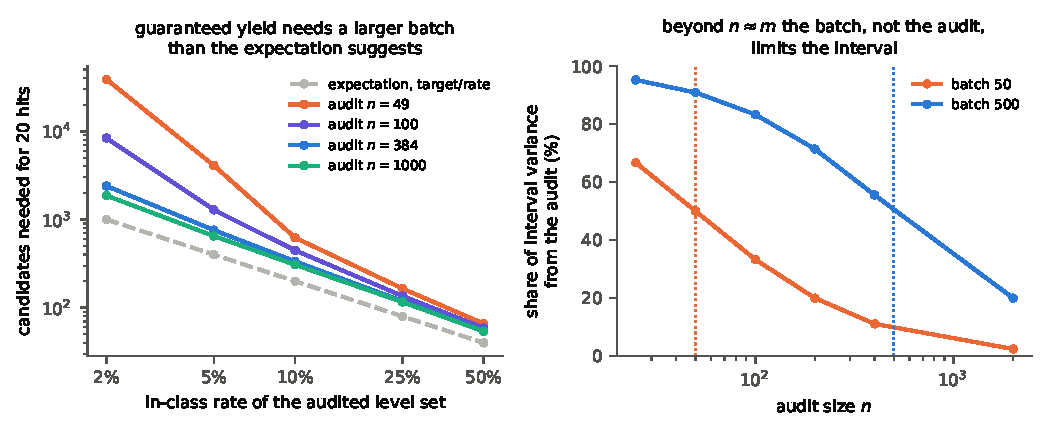
\includegraphics[width=\linewidth]{figures/fig9_sizing.pdf}
\caption{Sizing a round. Left: candidates the audited count implies for 20 hits at a confidence of 0.95, against the in-class rate of the audited level set, for four audit sizes; the dashed line divides the target by the rate, as an expectation does. Right: the share of an interval's variance contributed by the audit rather than by the batch, with the dotted lines marking where the audit matches the batch in size.}
\label{fig:sizing}
\end{figure}

The same intervals run backwards answer the question a campaign asks first: given a target
number of hits, how many candidates must the batch hold? The smallest batch whose lower bound
on confident hits reaches the target answers it. The interval is valid for each batch size
fixed in advance and the search makes the size a function of the audited count, so what follows
should be read as the size that count implies and not as a size carrying its own guarantee;
ESI Section~\ref{esi-sec:intervals} gives the convention, which is one-sided, and the
qualifications.

The answer differs from the one an expectation gives, and most where screens operate
(Fig.~\ref{fig:sizing}). Dividing the target by the observed rate, which is what a sum of
calibrated probabilities amounts to,\citep{Buendia2019Hit} asks for 1000 candidates to obtain
20 hits at a rate of 2\%. The audited count implies 2056 on an audit of 384 and 1687 on an
audit of 1000; at a rate of 50\% the expectation asks for 40 and both audits give 52. Three
quantities are stacked in that gap and separating them is what makes it planable. Were the rate
known exactly, 1390 candidates would still be needed, because which candidates fall in this
particular batch is not something measurement can settle. Knowing the rate from an audit of 384
raises it to 2056, and from an audit of 49 to 19\,091. The first is the risk the campaign
carries; only the second and third are for sale. A team planning on the expectation omits all
three.

At these rates the requirement is better read as a distribution than as a number: an audit of
49 at a rate of 2\% sees no in-class compound with probability 0.37, in which case no batch size
reaches the target at all. Enlarging the audit from 49 to 384 removes that possibility and
roughly halves the typical requirement. On this accounting the audit is the measurement with the largest effect on what the campaign costs, and not an overhead upon it, and its effect
is largest exactly where a screen's hit rate is low.

How much is worth buying can be settled before any compound is measured. Accepting a width $r$
times the narrowest any audit could achieve requires $n=m/(r^2-1)$ audit candidates, a ratio
independent of the rate and of the batch size: an audit the size of the batch lands a factor
$\sqrt2$ above that floor, one of $2.3m$ within 20\% of it. The floor itself depends on the
rate and at primary-screen rates it is wide. For a batch of 1000 at 2\% it is $\pm9$ on an expected 20, so a team should read the floor first and enlarge the batch, not the audit,
when the floor is what binds. Correlated series change the two statements differently: the
floor is a width and inflates by the square root of the design effect, while the ratio rule
needs no inflation, since the design effect multiplies both variance terms and cancels from
$r$.\citep{Cochran1977,Kish1965}

We can put numbers to that. The label's intracluster correlation is 0.60 for the electrolytes at
the level of the salt--solvent system, over the 138 systems that carry a room-temperature
formulation, 10.8 formulations each, hence a design effect of 6.9: the 1495 formulations are
worth about 220 independent ones. For the library at the first-position block the correlation is
0.35 with 680 molecules per block, a design effect of 238, so the 200\,000 analysed are worth
about 840. What this touches is worth separating, because it touches less than it appears to. It
does not touch the intervals: the construction conditions on the total count in the audit and
batch together, which absorbs the between-cluster variance, so under random assignment both
coverage and width are invariant to the correlation. Nor does it touch the ratio rule. Where it
bites is any statement that treats a count of candidates as a count of independent observations. Affected are the reach of a pilot, how many clusters a sweep has really explored, and the confidence due
to a coverage figure estimated from correlated splits.

Re-estimating the rate between rounds costs a seventh to a
quarter of a batch if the number of looks is declared in advance, and is not covered at all if
a campaign stops when the hits so far look sufficient; ESI
Section~\ref{esi-sec:intervals} states both conditions and the anytime-valid alternative.

\subsection{What a measurement budget costs: a solubility screen}
\label{sec:results:solubility}

\paragraph{The decision space.} Sweeping $(\alpha_0,\alpha_1)$ over 12 values each, with
$\delta=0.10$, gave 132--144 distinct settings per split, and their audited consequences range,
for one model and one endpoint, from 10 missed soluble compounds per 1000 with a third of the
batch sent to measurement to almost no measurements at the price of about 50 missed
(Fig.~\ref{fig:solubility}, left). Of those, 74--120 per split were Pareto-optimal for missed
compounds, false leads and measurements. A front that large invites the question whether it is a
decision surface or a restatement of the grid, and the answer depends on the objective:
minimising missed compounds selected the same request in eight of ten splits, while minimising
deferrals wandered over eight. The front is stable where the objective is steep and loose where
it is flat, so a team should read a setting's audited counts, not its coordinates
(Table~\ref{tab:solubility}). Because a setting chosen by looking at the audit carries the Bonferroni intervals instead of the pointwise ones, setting A's missed compounds are bounded at
$[0,49]$ and not $[2,29]$.

\paragraph{The price of a budget.} Two scenarios make the trade concrete
(Fig.~\ref{fig:solubility}, centre and right). In both, a batch of 1000 lipophilic compounds must
yield at least 60 confirmed soluble compounds and miss at most 90, the objective is the fewest
expected false leads, and the limits were set after inspecting the map, which the joint bounds allow, every constraint being checked at a level divided over the 144 requests and four bounded
outcomes so that all hold together at 95\%. Allowing 450 compounds to be measured, 26 requests
were feasible and the chosen setting expects 115 false leads and 286 measurements per 1000,
bounded jointly at 395 measurements and at least 66 confirmed. Tightening the budget to 250 left
9 feasible requests and a setting expecting 188: the tighter budget costs 73 additional false
leads per 1000. The gap between 286 expected and 395 bounded measurements is the price of the
guarantee at this audit size, and labelling buys it down. Half the audit would bound it at 432 and four times the audit at 358.

Those are one split, and the spread across ten is wide enough to matter: the number of
certifiable settings runs from 11 to 65 and the cheapest certifiable budget from 29 to 309 per
1000, with a median of 134. The setting chosen here is certifiable in only four of the ten
splits, so it is this split's choice and not a recommendation. The joint correction also costs
reach as well as width, the share of the grid meeting the limits falling from 0.2--0.6 read
pointwise to 0.0--0.1 read together, so a scenario that looks comfortably feasible on point
estimates can have almost no certified settings. What the screen does earn is the measurements it
saves: the compounds advanced without measurement were 54\% soluble against a prevalence of
22\%, an enrichment of 2.4 times on 51 of 95 compounds, significant after correction over the
sweep. Further detail, including the Pareto membership across splits and the cost-ratio map, is in
ESI Section~\ref{esi-sec:costs}.

\begin{table*}[t]
\centering
\caption{Audited consequences of two settings of the lipophilic solubility screen (split 0), per 1000 compounds: realized rate per 1000 in the audit set (384 compounds; 10 per 1000 is 4 observed compounds), with the 95\% prediction interval for a batch of 1000 and the interval with Bonferroni correction over the 144 requests of the sweep, which remains valid for one nominated outcome after choosing a setting by its audited outcomes. Holding all six lines of a chosen setting jointly would require the level divided by $144\times6$ instead; the scenario bounds quoted in the text are computed that way, over the four outcomes they constrain. A: the Pareto setting with fewest audited missed soluble compounds, ties broken by fewer deferrals, $(\alpha_0,\alpha_1)=(0.30,0.075)$; B: the Pareto setting with fewest audited deferrals, ties broken by fewer misses, $(0.275,0.25)$; $\delta=0.10$.}
\label{tab:solubility}
\small
\begin{tabular}{@{}lrccrcc@{}}
\toprule
 & \multicolumn{3}{c}{Setting A} & \multicolumn{3}{c}{Setting B} \\
 & audit & 95\% & Bonferroni & audit & 95\% & Bonferroni \\
\midrule
\inputrows{tables/tab_solubility_rows.tex}
\bottomrule
\end{tabular}
\end{table*}

\begin{figure*}[t]
\centering
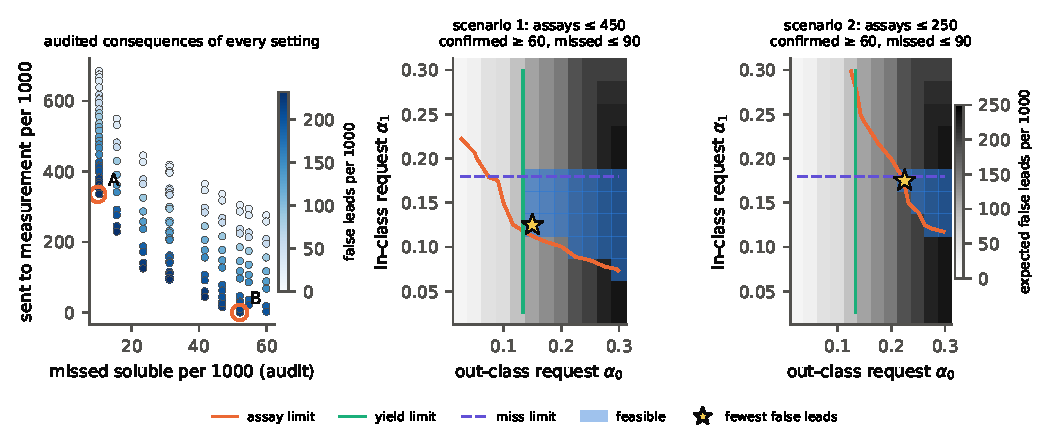
\includegraphics[width=\textwidth]{figures/fig7_solubility.pdf}
\caption{Navigating a solubility screen for lipophilic compounds (AqSolDB, $\log P>3.5$; split 0) with one model. Left: each point is one setting of the coverage requests, placed by its audited missed soluble compounds and measurements, with false leads in colour; A and B are the settings of Table~\ref{tab:solubility}. Centre and right: two scenarios in the plane of the coverage requests, with the expected number of false leads (grey, the objective) for each request. Lines mark where the 95\% joint bound of each constrained outcome equals its limit; blue cells satisfy all constraints with joint probability at least 95\%, and the star is the feasible setting with the fewest expected false leads. The right panel tightens the assay budget from 450 to 250 per 1000.}
\label{fig:solubility}
\end{figure*}

\subsection{One request, twelve sets of consequences: Tox21}
\label{sec:results:tox21}

After standardization and de-duplication, 7592 Tox21 compounds remained, with 5619--7017 labelled per endpoint and an in-class prevalence of 2.9--15.9\% among labelled compounds (the labels are missing non-randomly, which the Limitations quantify). Here a confident hit is a compound confidently flagged as toxic, which a screen would set aside. Calibration sets contained a median of 44--228 in-class compounds per endpoint (ESI Table~\ref{esi-tab:tox21data}). Audit AUROC was 0.70--0.87 for random splits and 0.67--0.85 for scaffold splits. These
endpoints also bound the decision-geometry reading of Section~\ref{sec:methods:choice}, which
needs the probability of being in-class to increase with the score. It does not here: the
in-class fraction decreases over at least one adjacent pair of score bins in nine of the twelve
endpoints, nominally so for two at $z=2.4$ and $2.6$, an uncorrected comparison that does not survive correction across the 108 bin pairs examined, and for three endpoints the fraction is
nearly flat over the lower nine bins with the signal confined to the highest (ESI
Table~\ref{esi-tab:tox21mono}). The containment argument and the cost-optimal reading therefore
do not apply to those endpoints, though the intervals themselves need no such condition. Before tie-breaking, a median of 3.3--4.3\% of scores were tied, mostly from identical fingerprints.

\paragraph{The same request, very different consequences.} All endpoints were calibrated with the same request, $\alpha=\delta=0.10$ per class, using the batch correction. Yet the median fraction of compounds receiving a single label ranged from 13.6\% (NR-PPAR-$\gamma$) to 62\% (NR-AhR) (Fig.~\ref{fig:tox21}). Table~\ref{tab:tox21cells} gives the audited consequences of the two extremes, for the split with the median single-label fraction. For NR-AhR, a batch of 1000 compounds yields 78 confident hits (audit interval 58--101) against 78 false leads (57--100). For NR-PPAR-$\gamma$, it yields 15 (6--26) against 89 (67--113), with 865 compounds deferred. Half of the toxic calls are correct for NR-AhR, one in seven for NR-PPAR-$\gamma$. The audit reveals these consequences before the screen is run. The fraction of in-class compounds among single-label ``in-class'' calls ranged from 13\% to 58\%, an enrichment of 3.0 to 6.5 times over prevalence. With the standard threshold the single-label fractions were larger, 28\% and 72\%, but that threshold's coverage of a class fell below the 90\% target in 41.5\% of the 600 endpoint--split pairs for in-class compounds and 47\% for out-class compounds, and in 54--80\% of splits per endpoint for at least one of the two.

\begin{figure}[t]
\centering
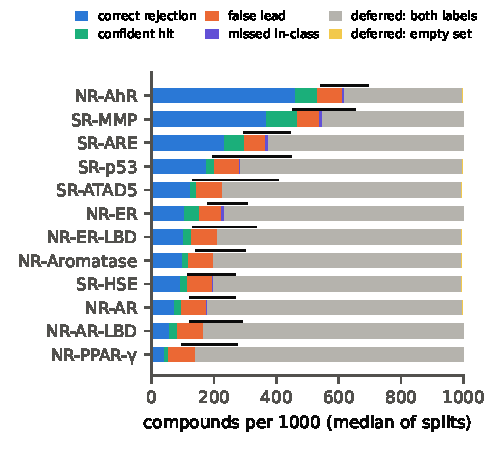
\includegraphics[width=\columnwidth]{figures/fig6_tox21.pdf}
\caption{Twelve Tox21 endpoints calibrated to the same request ($\alpha=\delta=0.10$ per class, batch correction) sort a screening batch very differently. Bars: median audited counts per 1000 compounds over 50 random splits, ordered by single-label fraction (medians need not sum to 1000); no empty sets occurred. Black lines: 5--95\% range of the single-label count over splits.}
\label{fig:tox21}
\end{figure}

\begin{table}[t]
\centering
\caption{Audited consequences per 1000 compounds for the endpoints with the highest and lowest single-label fraction (batch correction), for the random split with the median single-label fraction (25th of 50). Entries: realized rate per 1000 in the audit set, with the 95\% audit interval for a batch of 1000 in brackets. Calibration sets: 1385 out-class compounds and 197 in-class compounds (NR-AhR), 1526 and 37 (NR-PPAR-$\gamma$).}
\label{tab:tox21cells}
\small
\setlength{\tabcolsep}{4pt}
\begin{tabular}{@{}llrr@{}}
\toprule
True label & Outcome & NR-AhR & NR-PPAR-$\gamma$ \\
\midrule
\inputrows{tables/tab_tox21cells_rows.tex}
\bottomrule
\end{tabular}
\end{table}

\subsection{Auditing a new salt: an electrolyte screen}
\label{sec:results:calisol}

CALiSol-23 pools 13,825 conductivity measurements of lithium-salt electrolytes from 27
publications.\citep{deBlasio2024CALiSol} After the exclusions described in ESI
Section~\ref{esi-sec:molecular}, 1495 formulations had been measured at room temperature, 275 of
them (18\%) at or above the $8\,\mathrm{mS\,cm^{-1}}$ cut. That cut is close to the conductivity
of standard carbonate electrolytes, and close enough that the reference electrolyte straddles it:
the ten room-temperature measurements of 1\,M LiPF$_6$ in EC/EMC (3:7) here run from 7.85 to
10.21, and a quarter of all formulations sit within 20\% of the cut. That is the price of a binary
label on a continuous property recorded across sources, and it is the same price the solubility
screen pays. Measuring conductivity is cheap compared with building and cycling cells, so here a
deferral means a measurement.

\paragraph{A new salt.} The sharpest test holds out a whole salt. It is a weaker test than the name suggests: the salt held out is LiPF$_6$, which is the incumbent of commercial practice, supplies 606 of the 1495 room-temperature formulations, and anchors the class boundary, so what is tested is transfer to a well-represented salt instead of to novel chemistry; its share of good formulations, 25\%, also differs from the salts calibrated on, so prevalence moves with the chemistry here as it does in the library screen. A genuinely novel salt is not available in this compilation, where several candidates contribute a single room-temperature formulation each. With a model trained and calibrated on the other salts and the 606 LiPF$_6$ formulations screened, coverage of the good class averaged 29\% and fell below 90\% in all 50 splits (Table~\ref{tab:calisol}; Fig.~\ref{fig:calisol}, right). The audit of the screened formulations showed what this meant for the screen: at the default setting it reported a median of 174 missed good electrolytes per 1000 formulations, about two-thirds of the good ones, and 59 confident hits. Calibrating instead on a random pilot of 40\% of the LiPF$_6$ formulations, about 240 measurements, restored it for the good class (5 shortfalls against 3.3 expected) and left a residual excess for the poor class (8 against 4.0, one-sided Poisson-binomial $p=0.04$), and the audit showed the gain: 10 missed good electrolytes and 159 confident hits per 1000, for 308 measurements. Formulations split at random over all salts met the request (2 and 4 shortfalls against 4.7 and 3.1 expected), and the sweep of coverage requests gave 108--132 distinct settings per split, trading measurements (0--230 per 1000) against false leads (0--150) and missed good electrolytes (0--30) (Fig.~\ref{fig:calisol}, left). Holding out whole salt--solvent systems also broke the coverage guarantee (20 and 22 shortfalls against 4.5 and 5.0).

\paragraph{The audit carries the guarantee.} In all four designs, including the two in which the coverage guarantee failed, an audit set from the screened formulations reported the consequences correctly. Audit intervals for the default setting covered 95.5--100\% of realized counts, pointwise intervals over the whole sweep 97.2--97.6\%, and with the Bonferroni correction every setting and outcome was covered together in 98.4--99.2\% of audit--future splits. A capacity rule chosen on one audit half, as a planner would choose it, never exceeded capacity on the other half, in 980--1000 checks per design. The intervals were also informative: for the scenario setting the 95\% intervals were 12 to 63 times narrower than the trivial $[0,1000]$, and 7 to 28 times narrower jointly over the sweep. The advanced formulations were 71\% good against the 15\% prevalence of the audit set of the split these maps use, which is lower than the 18\% of the room-temperature compilation as a whole, an enrichment of 4.7 times (one-sided Fisher exact test on the audit set, $p=2\times10^{-37}$, Bonferroni over 144 settings). Scenario maps for the electrolyte screen behave as for solubility (ESI Fig.~\ref{esi-fig:calisolscen}). Intervals from the calibration set alone covered 99.7\% of counts for random formulations; for a new salt they rely on a calibration that does not match, and a separate audit is the tool to use.

\paragraph{Per plate.} A self-driving platform measures plates of 96, not batches of 1000. For the pilot-calibrated rule, an audit of 364 formulations gives, for one 96-well plate, 30 expected measurements with a 95\% interval of 20--40; scaled Clopper--Pearson would give 25--35, too narrow at this ratio of audit to batch size (Section~\ref{sec:results:intervals}). The one-sided bound of 38 measurements per plate holds with probability 95\% for a single plate, and a bound of 43 holds for all ten plates of a campaign together (level 0.5\% per plate).

\begin{table*}[t]
\centering
\caption{Electrolyte screen (CALiSol-23, conductivity $\ge8$\,mS\,cm$^{-1}$ at room temperature), 50 splits per design. Shortfalls: splits in which audit-set coverage of the class fell below 90\%, observed/expected under the exact law. Audit coverage: percentage of realized counts in the stand-in future batch covered by 95\% audit intervals, for the default setting (range over outcomes), for every setting of the sweep (pointwise), and for all settings and outcomes together with the Bonferroni correction over 144 requests.}
\label{tab:calisol}
\small
\begin{tabular}{@{}lrcccccc@{}}
\toprule
 & & \multicolumn{2}{c}{Shortfalls} & \multicolumn{3}{c}{Audit coverage (\%)} \\
Calibration and audit drawn from & AUROC & poor & good & default & sweep & Bonferroni \\
\midrule
\inputrows{tables/tab_calisol_rows.tex}
\bottomrule
\end{tabular}
\end{table*}

\begin{figure*}[t]
\centering
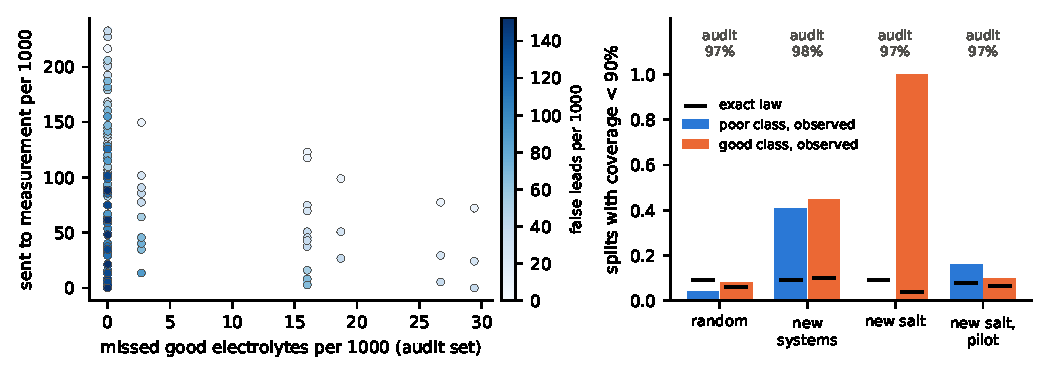
\includegraphics[width=\textwidth]{figures/fig8_calisol.pdf}
\caption{Electrolyte screen (CALiSol-23). Left: each point is one setting of the coverage requests for one random split, placed by its audited missed good electrolytes and measurements per 1000 formulations, with false leads in colour. Right: fraction of 50 splits in which coverage of each class fell below 90\%, observed (bars) and expected under the exact law (black marks), for calibration on random formulations, on other salt--solvent systems, on other salts, and on a pilot sample of the new salt; above each design, the pointwise coverage of the audit intervals over the sweep.}
\label{fig:calisol}
\end{figure*}

\subsection{An audit and a batch that are not two halves of one set}
\label{sec:results:source}

Every check of the audit intervals reported so far divides one labelled pool at random, which
makes the two halves exchangeable by construction and establishes that the construction is
right rather than that it survives a real separation. The electrolyte compilation lets the
harder question be asked, because it records which paper each measurement came from. We
therefore divided the formulations by source instead of at random, so that no paper
contributes to both the audit and the batch, holding the model and the calibration set fixed
across the divisions and halving nothing. The protocol is the one used elsewhere in this
paper: formulations are assigned to training, calibration and the remainder, the model is
fitted on every temperature row of the training formulations and is therefore disjoint from
the set that sets its thresholds, and the remainder is divided three ways.

The intervals do not survive it. Over ten repeats, random halving covered $0.97\pm0.04$ of
the consequence lines, as it must; partitioning the papers at random and letting each
formulation follow its own paper covered $0.70\pm0.12$; and taking one paper's formulations
as the batch and the rest as the audit, over the five papers large enough to serve within the
remainder, covered $0.77\pm0.11$. The inference here is about papers, so the paper is the
unit and not the repeat: the five per-paper means run from 0.58 to 0.90, and pooling the 41
runs instead would quote $\pm0.05$ and hide that spread. A division by provenance therefore costs
roughly a quarter of the coverage a random halving delivers, and nothing a campaign can
compute beforehand announces it. Area under the curve on the batch ran from 0.81 to 1.00
across these divisions. The enrichment of the confident calls, taken over the pool's base
rate, which is the rate a campaign knows, sits between 3.3 and 4.9 in all three divisions and
does not track coverage within any of them (Spearman $+0.01$ by source, $-0.19$ one source
out). The one quantity that does track coverage is the ratio of the audit's in-class rate to
the batch's, and that ratio needs the batch's labels, which is what the audit was to replace.

What the designs do not do is separate the causes. The median ratio of audit to batch
in-class rate is 1.02 halved, 0.67 by source and 1.88 one source out, and the per-repeat
ratios span 0.3 to 2.2 and 0.4 to 8.1 in the two source divisions. So dividing by provenance
moves the in-class rate as well as the mapping from score to outcome, and the coverage loss
is attributable to the two together. That is itself the practical point, since a paper is a population in both senses, although it means this experiment shows that provenance is enough to void the intervals, and not that the mapping alone is.

\paragraph{A pilot of the right population, divided for real.} The remedy this suggests is
the one the library screen also points to: when a round reaches into a population the audit
does not hold, buy a pilot of that population. Every arrangement reported so far that recovers
the nominal level divides one pool at random, which cannot fail, so none of them tests that
advice. The compilation lets it be tested, because a single paper's formulations can be
divided in ways that are not random. Holding the thresholds on the other sources throughout,
so that the rule is calibrated off-population exactly as a campaign would have it, we held out
one source as the screened population and varied only where the audit came from: from the
other sources, as a team would do by habit; or from the held-out source itself, divided by
concentration band, by solvent system so that no system is shared, or simply as the paper
reported its formulations, first half against second.

The advice holds. Taking the source as the unit, an audit drawn from the other sources covered
$0.55\pm0.07$ of the consequence lines over eight sources. A pilot of the screened source
covered $0.92\pm0.17$ when the division was by concentration, $0.87\pm0.21$ by solvent system
and $0.86\pm0.12$ as reported; on the sources that support both arrangements the paired gain
over auditing off-source is $+0.37\pm0.21$, $+0.37\pm0.26$ and $+0.34\pm0.17$. A random
division of the same source covered $0.99\pm0.02$, which is the ceiling the construction
guarantees and which these divisions do not quite reach: sampling the right population
recovers most of what provenance costs, and not all of it.

Two details are worth keeping. The divisions by concentration and by system leave the audit and
batch in-class rates close, at median ratios of 1.04 and 1.09, so this is not a prevalence
effect; the off-source arm sits at 0.56. And the division as reported, which is merely non-random and carries no chemical meaning, leaves the rates badly mismatched at a median ratio of 1.81
and still recovers to $0.86$. Sampling the population the batch comes from therefore helps even
where the prevalence does not match, which is the asymmetry the construction predicts: what the
audit must share with the batch is the mapping from score to outcome, and a prevalence gap it
can report.

Two things follow. The first is a limit on this work's own evidence: the coverages quoted
for solubility, toxicity and electrolytes under random splitting are verification, and the
only divisions in this paper that test the intervals against a genuinely distinct batch, these together with the library's block holdouts, break them. The second is a limit on pooled
compilations, which is where much of the data for materials screening comes from. An audit
drawn from the library to be screened is not sufficient if the batch will be measured by
someone else, on another instrument, with another calibration: provenance is part of what
must be exchangeable, and a compilation of 25 papers is 25 populations. The instruction to
audit the population you will screen therefore extends to the laboratory that will screen it.

\subsection{Building the audit for the round it prices: a DNA-encoded library}
\label{sec:results:del}

The electrolyte screen showed that an audit drawn from the screened population bounds the
consequences where a calibration set from elsewhere does not. A campaign poses a harder version,
because the next round often introduces chemistry that has not been made. What the audit must
then contain is a question about its design, and a DNA-encoded library answers it cleanly: the
chemistry is built from a catalogue of building blocks, so a round can be declared in those
terms.

\paragraph{What a structural split costs.} Assigning molecules to training, calibration, audit
and batch at random keeps all four exchangeable, and the intervals covered 53 of 54 consequence
lines over nine repeats. Withholding instead every molecule carrying a given block at one
position, so that the batch is built on chemistry absent from the calibration and audit sets,
breaks them. Taking the repeat as the unit, since the six lines of one repeat are cells of a single table on a single batch and not independent checks, coverage was $0.48\pm0.19$, $0.37\pm0.14$ and
$0.35\pm0.12$ for the third, second and first positions, against $0.98\pm0.04$ for random
assignment. Over the same runs the model's ranking fell only from 0.960 to 0.892 by area under
the curve. This is the split a project adopts to guard against memorisation, and passing it
licenses nothing quantitative about the next batch.

Nothing a campaign can compute beforehand orders these failures. Area under the curve is
governed by the ordering of the negatives at a sub-percent rate and is invariant to prevalence by
construction, so it cannot announce a prevalence change. The enrichment of the confident calls,
which a screening group reports as a matter of course, is the audit's own in-class rate re-expressed, dividing the precision of those calls by exactly that rate, and within the
first-position repeats it does not order them by coverage: its largest value belongs to a repeat
covering three of six lines, while the repeat covering none sits mid-range. The audit's rate
against the library's is a cheap partial warning and not a test: pooled over the thirty
block-holdout repeats it predicts coverage only moderately, and within the first position not at
all (ESI Section~\ref{esi-sec:del}). What does predict coverage is the audit's rate against the
\emph{batch's}, which needs the batch's labels.

These designs move the in-class rate of the audit and of the batch independently, between 0.2\%
and 2.5\%, because in-class molecules are concentrated in a few blocks. So the losses are a
change in prevalence as well as a change in the mapping from score to rate, and the designs do
not separate the two; the arm that holds matches the batch's prevalence by construction. Dealing
blocks to the four roles in order of their in-class count would separate them while keeping the
design block-disjoint, and we have not run it.

\paragraph{A declared round.} A round is declared in which 30\% of the batch is built on
first-position blocks the model has never seen, and three preparations are compared, each
supplying its own calibration and audit sets and all three sharing one model per repeat:
calibration and audit from familiar blocks only, as a team would do by habit; from different new
blocks but at the batch's own 30\% share, which is where a team stands that has measured some new
chemistry and is about to make different new chemistry; and from the batch's own new blocks,
which is a pilot of the chemistry the round will contain.

Reproducing the batch's composition is worth nothing. Familiar blocks covered $0.63\pm0.13$ of
the consequence lines and the batch's proportion of new chemistry from other blocks covered
$0.63\pm0.10$; because those two arms share a batch and nearly nested audits their difference can
be taken per repeat, and it is $0.000\pm0.070$, which is the strongest form of the claim. Neither
comes near the request. Sampling the batch's own blocks covered $0.97\pm0.04$ and was the only
arrangement to cover all six lines in a majority of repeats, eight of ten against one and none. That arm, however, splits a fixed pool at the molecule level, which makes its calibration, audit
and batch exchangeable by construction, so its 0.97 is a positive control rather than evidence
that a pilot repairs a campaign. Its narrower interval is likewise a property of its audit being
43\% larger and not of the arrangement (ESI Section~\ref{esi-sec:del}).

What distinguishes the three is therefore whether the audit holds \emph{that} chemistry, and not how much new chemistry it holds. The first is cheap and can be arranged before synthesis; the
second requires measuring a sample of the new blocks, which is an experiment. Both arrangements
that do not sample the batch's own chemistry fail, and none short of sampling it was found to
work.

\subsection{The batch the model chose}
\label{sec:results:adaptive}

Every division so far has been random or structural. A campaign is neither: a planner reads
the scores and commits the top of the ranking, which is the one arrangement this construction
is not expected to price. We tested it on the library, holding the model fixed so that only
the selection moves. A pool of 70\,000 candidates was scored, the planner committed the
highest-ranked $m$ of those remaining in each round, and the same committed batch was priced
three ways: with a random sample of the candidates still in the pool, which is the audit a
team would reserve; with a random slice of the committed batch itself, measured and used to
price the remainder; and with the same selection rule applied to a pool of 20\,000 reserved
from the planner. Two round sizes were run, $m=8000$ and $m=1500$.

The audit reserved from the library does not price a plate the model chose, and the reason is
visible before any interval is computed. In the first round at $m=1500$ the committed batch
had an in-class rate of 0.269 against 0.0071 for the pool it was drawn from, a factor of 38;
what remained of the pool fell to 0.0013. Across the twelve rounds of the two campaigns the
library audit could not even be formed in nine, because a sample of the leftover pool
contained no in-class candidate at all, and in the three rounds where it could be formed it
covered 2, 2 and 4 of the six consequence lines. A quantity that cannot be estimated is a
safer failure than one estimated wrongly, but neither is a guarantee. The usual repair for a
covariate shift is to reweight the calibration sample by the likelihood ratio between the two
populations,\citep{Tibshirani2019Weighted} which requires that ratio to exist and to be known
or estimable. A planner that commits the top $m$ of a ranking does not shift the population
smoothly; it concentrates it on a set chosen by the same score the rule thresholds, and the
weights such a selection would need are unbounded on it.

Both repairs work, and the first is exact. A random slice of the committed batch covered all
six lines in every one of the nine rounds in which it could be formed, which is what the
construction requires: a random division of a committed set is exchangeable with the rest of
that set however the set was chosen, so the selection drops out. Applying the selection rule
to a reserved pool also worked, covering all six lines in eight of ten rounds and four of six
in the other two; it is an approximation rather than an identity, since the reserved pool and the screening pool are two draws and not one, and it costs a pool of high-scoring
candidates the planner may not commit. The three rounds in which the batch was rich enough for
the comparison to carry weight, at batch rates of 0.269, 0.055 and 0.020, show the pattern
most clearly: library audit unavailable, 2 of 6 and 2 of 6; batch slice 6, 6 and 6; reserved
selection 6, 4 and 6.

The second finding concerns the sequence of rounds and not a single one, and it is the one that bounds
what any audit can do for a campaign. One round exhausts the library. Committing 1500 of
70\,000 candidates, 2\% of the pool, took the in-class rate of the remainder from 0.0071 to
0.0013, and committing 8000 took it to 0.0005; by the fifth round of the smaller campaign no
arrangement could be formed at all, because nothing in-class was left to sample. So a round's
audit does not price the round after it even with the model frozen, the rule fixed and the
selection unchanged, and not because the mapping from score to rate has moved: the population
underneath has been removed. An audit is a measurement of the library as it stands, and at a
sub-percent in-class rate a single round changes the library it measured. The instruction that
follows is to reserve a slice of every committed round instead of amortizing one audit over a campaign, which is cheap, and to read the falling rate of the remaining pool as the campaign's
own statement about how much is left to find.

\subsection{Checking exchangeability before the batch is made}
\label{sec:results:preflight}

The preceding result is a design instruction, and a team following it would like to know whether it has succeeded. Exchangeability binds the calibration set, the audit set and the batch, and all three are sets of structures that exist before any of them is assayed, so the question can be put to the structures alone. We ask it as a two-sample problem: a classifier is trained to tell audit compounds from batch compounds using fingerprints and no labels. That is the pair the predicted counts depend on, since the audit prices whatever rule it is handed and asks only to be exchangeable with the batch; the calibration set may be compared with the batch in the same way when the coverage guarantee is also wanted. Under exchangeability the two are draws from one distribution, no classifier can separate them, and its area under the curve sits at one half.

Run across the four split designs, the test separated every arrangement that later failed and did not separate the one that held (Table~\ref{tab:preflight}); what it can refute is bounded by the representation, as the end of this section and the Limitations set out. It sits at 0.498 for random assignment, which covered 98\% of consequence lines, and at 0.985, 0.989 and 0.997 for the three block holdouts, which covered 48, 37 and 35\%; comparing the calibration set with the batch instead gives 0.501, 0.987, 0.990 and 0.999, so on these designs either pair would have raised the alarm. Beside it we report the share of batch molecules whose block at each position also occurs in the comparison set, which is the quantity the design controls directly. That share is one everywhere under random assignment and falls to zero at exactly the withheld position in each holdout, so the two statistics together give a verdict and name the axis responsible.

Those four designs are the easy case, and the table should be read as a check that the test fires and not as a measure of its sensitivity: a withheld block catalogue is a substructure a fingerprint represents directly, so a classifier must find it, and the block-share column gives the same verdict by inspection. The question that matters is whether the test sees the three preparations of the declared round, which differ not in how much novel chemistry the batch carries, all three holding 70\% of their batch's first-position blocks, or all of them for the pilot, but in where the audit draws its own. Over two repeats the audit-against-batch area under the curve was 0.658 for the naive preparation and 0.663 for the mirror, against 0.502 for the pilot; over the ten repeats of the coverage experiment the first two cover 38 of 60 consequence lines each and the pilot 58 of 60. The permutation null, obtained by shuffling the audit and batch labels and refitting at the same cap as the statistic itself, averaged 0.500 over 120 replicates and spanned 0.491 to 0.511, so the two preparations that fail are separated from the null by a wide margin and the one that holds lies inside it. The test therefore distinguishes arrangements that a fingerprint comparison of composition cannot, which is what the workflow step requires of it.

The test is one-sided and should be read that way. Separation is strong evidence against exchangeability, because two samples from one distribution cannot be told apart. Failure to separate is weak evidence for it, since a classifier may simply lack the features to see a difference that matters; the fingerprints used here cannot distinguish stereoisomers, for instance, whose in-class rates in this library differ severalfold. A screen that passes is therefore uncertified, although a screen that fails is refuted, which is enough to be worth running: it costs no measurements, uses structures already known, and can be run before the plate is committed. The clearest case it cannot see is the provenance division of Section~\ref{sec:results:source}: which paper a measurement came from is not a property of the formulation, so no test on structures can detect a division that costs roughly a quarter of the coverage. At the first position of this library, 60 of the 294 blocks form 30 pairs that are stereoisomers, indistinguishable under the achiral fingerprint used here and differing severalfold in in-class rate; that is a fifth of the catalogue carrying most of the binders, invisible to the test by construction.

\begin{table}[t]
\centering
\caption{A label-free check, run on structures alone before any compound is assayed, against the coverage each design later achieved. The domain classifier separates audit compounds from batch compounds, which is the pair the predicted counts require; one half means they cannot be told apart. The block shares are the fraction of batch molecules whose building block at each position also occurs in the audit set.}
\label{tab:preflight}
\small
\setlength{\tabcolsep}{4pt}
\begin{tabular}{lccccc}
\toprule
 & domain & \multicolumn{3}{c}{block share at position} & \\
\cmidrule(lr){3-5}
split design & classifier & 1 & 2 & 3 & cov. \\
\midrule
random assignment & 0.498 & 1.00 & 1.00 & 1.00 & 98\% \\
withhold pos.\ 3 & 0.985 & 1.00 & 1.00 & 0.00 & 48\% \\
withhold pos.\ 2 & 0.989 & 1.00 & 0.00 & 1.00 & 37\% \\
withhold pos.\ 1 & 0.997 & 0.00 & 1.00 & 1.00 & 35\% \\
\bottomrule
\end{tabular}
\end{table}

\subsection{When the label is not the one the claim concerns}
\label{sec:results:surrogate}

The audit sections asked which compounds a round must measure. The same assumption can fail
along the other axis: the compounds may be interchangeable while the label recorded on one set is
not the label recorded on another. A campaign calibrates against what it can afford, such as a selection count, a cheaper assay or a single-concentration readout, and claims something about
the endpoint it cares about. One case is free: no part of the rule reads the score's value, only
its order, so any strictly increasing relabelling of the truth at matched prevalence leaves every
cell of the outcome table unchanged, which we verified cell for cell on three scales (ESI
Section~\ref{esi-sec:surrogate}). Real proxies are not increasing functions of anything. What governs the shortfall is local, and follows from the construction: the threshold sits at a fixed quantile of the score distribution conditioned on the \emph{proxy's} label, whereas the coverage achieved is the score distribution conditioned on the \emph{true} label evaluated at that same threshold. The coverage achieved therefore decomposes into three terms,
\begin{equation}
\text{achieved} \;=\; (1-\alpha) \;+\; \bigl(\ell - (1-\alpha)\bigr) \;+\; \Delta,
\label{eq:gap}
\end{equation}
in which $\ell = F(\tau \mid \text{proxy out-class})$ is the realized level of the order statistic the threshold sits at and $\Delta = F(\tau \mid \text{true out-class}) - \ell$ is what the proxy costs. The middle term is the overshoot the batch correction introduces on purpose, and it is not small: the control below, whose proxy is the truth, measures $\ell = 0.924$ against a request of 0.90. Only the third term involves the proxy, and no part of it counts how many compounds the two labels disagree about. Measuring $\Delta$ against the control and not against the nominal level is what the agreement quoted below tests; the decomposition itself is an accounting identity. Disagreement costs coverage only insofar as it is structured with respect to the score.\footnote{Which is why a global summary of agreement, or a correlation between the proxy and the affinity, is the wrong thing to require of a proxy, and why comonotonicity is the right thing but is needed only locally: what Eq.~\ref{eq:gap} asks is that an isotonic regression\citep{Ayer1955Isotonic,Zadrozny2002Isotonic} of the affinity on the proxy be increasing over the narrow score region where the thresholds fall, which the rule itself identifies as the region in which it declines to commit to a single label. Away from that region a proxy may misorder compounds freely. Fitting such a mapping needs compounds measured both ways, which a campaign can buy on a small sample; inference that corrects a cheap proxy using exactly such a small gold-standard sample is the subject of prediction-powered inference,\citep{Angelopoulos2023PPI} which repairs the bias where the account here instead characterizes when there is none to repair.}

Three carbonic anhydrase isoforms let the mechanism be separated, because selection counts and
measured inhibition constants are published for the same
targets.\citep{He2026CADEL,Zdrazil2024ChEMBL} No molecule in that release carries both, so the
proxy is constructed from the affinities; what follows is therefore a demonstration of the mechanism and not a measurement of any assay's fitness. Varying only the calibration label, we
compare a strictly increasing relabelling at matched prevalence, which is the control, against
two proxies that relabel the same fraction of each class, one choosing those compounds uniformly at random and the other choosing the ones the score ranks most extremely against their
class. Their error rates, their ranking of the truth and the prevalence they imply are all equal;
they differ only in where their mistakes sit (Table~\ref{tab:surrogate}).

They behave nothing alike. At a fifth of each class relabelled, the random proxy left class-conditional coverage at 0.933 and 0.938 against a request of 0.90, falling short in 18 of 240 class-repeats, while the score-structured proxy gave 0.721 and 0.721 and fell short in 240 of 240, at every isoform and both cut-offs. Equation~\ref{eq:gap} accounts for this, and measuring both of its sides in the same run agrees to within 0.004 on average and 0.011 at worst across all 36 conditions: that is a consistency check on the accounting and not a prediction, and its value is that it locates the quantity and not that it is accurate. The audit-set intervals, meanwhile, covered 95.2\% of consequence lines over every condition, against their nominal 95\%, and are within Monte Carlo error across the table. They ask only that the audit and the batch be exchangeable and not that the rule be well calibrated, so they price whatever rule they are handed; a campaign that calibrates on a proxy keeps its predicted counts and loses its coverage guarantee, and only the audit tells it so.

\begin{table}[t]
\centering
\caption{Calibrating against a proxy label on three carbonic anhydrase isoforms, at affinity cut-offs of 7 and 8, 20 repeats each. The two proxies relabel the same fraction of each class and so agree with the truth equally well by any label-only summary; they differ in whether their mistakes are placed at random or where the score ranks compounds most extremely; the rows below name that placement. Coverage is class-conditional against a request of 0.90, pooled over isoforms and cut-offs; shortfall counts are given in the text rather than as a column.}
\label{tab:surrogate}
\footnotesize
\setlength{\tabcolsep}{4pt}
\begin{tabular}{lccccc}
\toprule
 & relabelled & agree & \multicolumn{2}{c}{coverage} & audit \\
\cmidrule(lr){4-5}
proxy label & share & w/ truth & out & in & intervals \\
\midrule
increasing in affinity & 0.00 & 1.000 & 0.924 & 0.923 & 96\% \\
at random & 0.05 & 0.950 & 0.929 & 0.933 & 95\% \\
by score  & 0.05 & 0.950 & 0.873 & 0.872 & 95\% \\
at random & 0.10 & 0.900 & 0.932 & 0.936 & 96\% \\
by score  & 0.10 & 0.900 & 0.822 & 0.824 & 94\% \\
at random & 0.20 & 0.800 & 0.933 & 0.938 & 95\% \\
by score  & 0.20 & 0.800 & 0.721 & 0.721 & 95\% \\
\bottomrule
\end{tabular}
\end{table}


\paragraph{The same axis, on a real label.} The solubility screen above supplies the measured
counterpart. Its label cuts a continuous property recorded across sources, so it is noisiest
where it matters, at the cut: about 8\% of the screened compounds near it would be labelled the
other way by another laboratory, which is the size of the requests being swept. Re-running that
whole analysis on the same scores with only the labels changed shows what survives. The
resolution of the sweep does, and so does the enrichment, at a fold between 1.51 and 3.61 and
significant after correction in every one of a hundred perturbed evaluations, so an enrichment
of about twice the base rate is safe and the two digits of 2.4 are not. The scenario does not:
certifiable settings fall from a median 26 to 18 under random flips and to 2 and 0 under the two
adversarial variants, the cheapest certifiable budget rises by a factor of 2.2 to 2.8, and about
a quarter of the Pareto front is an artefact of the labels.

One direction of that perturbation runs against the mechanism just described, and is the sharper
form of it. Flipping the compounds the score ranks \emph{most} extremely, which is the structured case, \emph{flatters} the screen: more settings become certifiable, the enrichment rises and the
budget floor falls, because noise correlated with the score makes the recorded labels agree with
the model. The damaging direction is its mirror image. So score-structured label noise is not
ruinous in itself; its sign decides, and a proxy that agrees with the model conceals its own failure instead of revealing it (ESI Section~\ref{esi-sec:noise}).

\subsection{What the audit must sample}
\label{sec:results:dependence}

Two further checks show the same requirement from the calibration side, and one of them fixes
the attainability floor the workflow depends on. On Tox21 scaffold splits, calibrating on other
scaffolds broke the coverage guarantee, since per-class coverage fell short in 28\% of splits for
out-class compounds and 18\% for in-class, two to three times the exact-law expectation, while an audit from the screened scaffolds still reported the consequences correctly
(Table~\ref{tab:audit}), and calibrating instead on a random pilot of the screened scaffolds
restored coverage to the exact law. Calibrating on all compounds and then screening only the
lipophilic ones did the same thing in miniature: coverage of the soluble class averaged 72\%
there. A simulation in which compounds share scaffold-level shifts of their predicted probability
reproduces both, with coverage at 95.4--97.9\% when the audit samples the scaffolds being screened
and 62--75\% when it does not (ESI Section~\ref{esi-sec:sim}).

The attainability floor follows from the same arithmetic and is what step one of the workflow
rests on. A request at $\alpha=\delta=0.10$ cannot be met unless the calibration set holds at
least 22--23 compounds of the rarer class, so a pilot of $22/\pi$ randomly chosen compounds at
prevalence $\pi$ reaches it only about half the time and one of about $28/\pi$ nine times in ten.
At a primary screen's rate of 0.1--1\% that is thousands of measurements before the method
starts, which is the scope boundary of the library-reserved audit and the reason the
committed-batch slice of Section~\ref{sec:results:adaptive} matters: it is the only arrangement
here that does not pay it.

\section{Discussion}
\label{sec:discussion}

The audit turns a conformal classifier into a forecast: before a batch is screened, it predicts how many hits, false leads, misses and measurements the batch will contain, with intervals that hold at a stated probability. The two class-wise coverage requests move a conformal classifier through the decisions available to a screening team, and for every setting the consequences are counts in one outcome table: compounds advanced, discarded and deferred, and how many of those calls are wrong. Linked to these counts by the audit, coverage becomes a coordinate a team can steer by. An objective, usually with guarantees on what a campaign will consume and deliver that hold with a stated probability, decides where to steer. The coverage plane is where such scenarios are explored, and an audit set from the library to be screened supplies the consequences, with finite-sample valid intervals that remain valid after the team has chosen a setting by looking at them. On Tox21, AqSolDB and CALiSol-23 the intervals held at their nominal level, also when the calibration came from other scaffolds or other salts, the audit having come from the screened compounds. Those checks verify the construction rather than establishing that it survives a separately assembled batch, which is taken up below.

\paragraph{Using the method in a screen.} The results suggest the following workflow.

\begin{enumerate}\itemsep1pt
\item Label a random sample of the library as the calibration set. A request at
$\alpha=\delta=0.10$ needs at least 22--23 compounds of the rarer class to be attainable at all,
and about $28/\pi$ randomly chosen compounds at prevalence $\pi$ to reach it nine times in ten.
Picking compounds by score to find the rare class faster breaks exchangeability unless the
selection is accounted for.\citep{BarberBeyond2023}
\item Label a second random sample as the audit set, and choose its size from the width the decision needs, since any size delivers validity. Read the floor first: no audit
narrows an interval below $\pm2\sqrt{m\,p(1-p)}$, and accepting $r$ times that floor needs
$n=m/(r^2-1)$, so an audit the size of the batch is the natural place to stop
(Section~\ref{sec:results:sizing}).
\item Draw it from the chemistry the next batch will contain, not merely in the same proportion.
Where a batch introduces blocks, scaffolds or series the audit does not hold, a pilot of that
chemistry is the indicated step (Sections~\ref{sec:results:source} and \ref{sec:results:del}).
\item If the batch is selected by a planner and not drawn at random, reserve the audit from
the committed batch itself and re-draw it each round
(Section~\ref{sec:results:adaptive}).
\item Before committing, check that calibration, audit and batch cannot be told apart from
structures alone. It costs no measurements, and it withholds approval from an arrangement without ever certifying one (Section~\ref{sec:results:preflight}).
\item Sweep the requests and audit each setting, then state a scenario, being an objective together with the limits that must hold with probability $1-\varepsilon$, and read the feasible settings off the
map, with the bounds computed so that all of them hold together.
\item Screen, and compare the realized counts with the predicted intervals as a standing check on
exchangeability.
\end{enumerate}

\paragraph{The audit decides which questions can be asked.} Calibration and audit sets are usually treated as machinery, chosen for size and then forgotten. They are better understood as the statement of what the guarantees are about, because a sample licenses claims about the population it was drawn from and about nothing else. How the audit is built therefore fixes, before any model is fitted, which questions a campaign can answer, and three choices in building it each foreclose something. The population fixes the domain: an audit drawn from the top of a ranking prices further batches drawn from the top of that same ranking, and says nothing about compounds further down, which is where a campaign goes once the top is exhausted. The unit fixes what a count means: an audit sampled one compound per series estimates the rate at which series are real and prices a batch of new series and not a batch of analogues of a few confirmed ones, whose effective size is the number of series it contains. The chemistry fixes the reach: an audit holding only building blocks already screened prices batches built from those blocks, and carrying the same proportion of new chemistry as the batch without sampling that chemistry is not a substitute (Section~\ref{sec:results:del}). The label fixes the claim: what must be exchangeable is each candidate together with its recorded label, so a campaign that sets its thresholds against a cheap readout has made a statement about that readout and not about the quantity it cares about, however interchangeable the compounds are (Section~\ref{sec:results:surrogate}). The score belongs to the same declaration, since thresholds and the sets they define move when the model is refitted, so an audit describes the deployment it was measured under.

Reading the four together makes the condition less forbidding than it first appears, because exchangeability is sufficient but more than is needed. A coverage request concerns one quantile, and what the request actually buys is an agreement between calibration and batch at the cut it induces; a discrepancy elsewhere in the ranking is free. That is why a proxy whose errors fall away from the cut costs nothing while one whose errors fall on it is ruinous at the same error rate, and it suggests that the familiar violations might be graded the same way, by where in the ranking a population differs, and not by whether it differs at all. We have tested this only on the label, where the structure of the discrepancy can be set deliberately; doing the same for a change of chemistry would ask how much of the loss under a block holdout is attributable to the neighbourhood of the thresholds, which the designs here do not separate.

Two consequences follow for practice. The question should be settled before the audit is built, because an audit assembled for one question usually cannot be repurposed for another; a campaign that discovers halfway through that it needs to speak about a different population has to measure again. And because an audit is also an option on the questions a campaign may ask later, it is worth spending part of it on compounds a project would not otherwise measure, lower-ranked compounds or a few members of each of several series, so that when the obvious batch is exhausted the next question can still be answered. Diversity in an audit purchases future questions, and is no mere statistical nicety.

\paragraph{Campaigns run batch by batch.} Automated and self-driving laboratories synthesize and
characterize in parallel, so their campaigns are sequences of batches with fixed capacity, and
the construction applies to each batch as it stands. Three features of that setting make counts
the right object. The constraints are physical and integer, at 96 or 384 wells, a reagent budget and a minimum yield to justify the next round, and a scheduler cannot act on a rate; it needs the
probability that this plate exceeds capacity. The batches are small and frequent, which is the
regime in which the draw of the batch dominates the uncertainty, so the gap between a rate and a
count is widest here. And the audit is affordable, because reserving a slice of a committed plate spends candidate slots instead of a round.

The batch is a selection from a scored library under fixed capacity, however that selection is made, whether by rank, by a diversity-penalised acquisition, by space-filling or by a multi-objective front.\citep{Gonzalez2016LP,HernandezLobato2017TS,Shields2021EDBO,Joseph2016SFD,Kusne2020CAMEO,Eriksson2019TuRBO,Daulton2020qEHVI}
The outcome table accounts for which prediction set a candidate receives and not for how its batch was assembled, and $m$ is the plate or run size. But a planner that fills a plate from the top of
a ranking does not draw a random sample of the library, so an audit reserved from the library does not price that plate. Section~\ref{sec:results:adaptive} measures this instead of assuming it, and it fails for a reason visible without any model: the plate is several times richer than the
collection it came from. The repair is to sample the plate and not the library, and it is exact,
because a random slice of a committed batch is exchangeable with its remainder however the batch
was chosen, so the acquisition function drops out of the argument and needs no correction. The
rule a scheduler follows is therefore short and independent of how it chooses: reserve a random
slice of each committed round, price the remainder with it, and draw a fresh slice next round.
The third clause is not optional. One round at a sub-percent hit rate removes most of what was there to find, so an audit prices the round it came from and not its successor, and the falling rate of the remaining pool is itself the campaign's statement about how much is left. When the
model is retrained the thresholds change, so calibration, audit and map are redone for the new
deployment; the guarantee holds per batch at $1-\varepsilon$, and a statement over all $K$ batches
needs $\varepsilon/K$ each. Because the bounds are counts they can be checked automatically, and
the Pareto table is a menu a planner, including an AI agent, can choose from without a cost ratio
being stated; we do not test such a planner here.

\paragraph{Why the round, and not the candidate, is the unit.} Automated campaigns are often
pictured as sequential loops that adapt after every experiment, and such a loop corrects its own
errors whether or not its uncertainty was calibrated. Laboratories do not work that way, because
the cost of an experiment is dominated by the round: a plate, a synthesis run or an instrument
cycle costs nearly the same full or half empty, so cost rises in steps between rounds and barely
at all within one. Two consequences follow. An audit is cheap, because reserving part of a committed batch spends candidate slots instead of an extra round. And parallelism and predicted
consequences are complements rather than alternatives: a laboratory that could run one cheap
experiment at a time would have little use for an interval on a batch, while one that must
commit several hundred wells at once has the most use for one. A committed batch is then an
allocation under fixed capacity, divided between the candidates a setting advances and the random
sample that prices the round after it.

\paragraph{Limitations.} The serious objection is one sentence: every positive coverage
result in this paper divides one labelled pool at random, which verifies the construction and
cannot fail, and the two divisions that test it against a genuinely separate batch, by provenance and by building block, break it. The repairs reported above are the answer to
that, and one of them, the slice of a committed batch, is exact and not empirical; but a
reader should weigh the negative evidence as the stronger half.

Everything else follows from the precondition. A change of chemical series, scaffold or assay
breaks it, and so does calibrating against a label other than the one the claim concerns, which
breaks it without touching the composition of any set. A library proposed by a generative model
or extended into new chemistry breaks it, as the new-salt screen
shows;\citep{Fannjiang2022FeedbackCovariateShift,BarberBeyond2023} methods for shifted data are
complementary. A structural check does not substitute for a pilot: we found no relation between
how well an interval covered and how similar the held-out blocks were to those the audit held,
and blocks indistinguishable by fingerprint gave the lowest coverage of all, being stereoisomers
whose in-class rates differ severalfold. The same limit bounds the pre-flight test, which
inherits whatever the representation cannot see, the provenance division of Section~\ref{sec:results:source} being exactly such a shift, so a verdict can only decline an arrangement, never vouch for one.

Simultaneity and scope. Each interval covers one outcome of one setting, and statements about
many need the Bonferroni correction: with 144 requests and four bounded outcomes the joint
guarantee cost about 110 measurements per 1000 at an audit of 384, which larger audits lower and
an envelope valid simultaneously over thresholds would lower
further;\citep{Song2026FDP} Simes aggregation over a batch dominates Bonferroni
uniformly\citep{Gazin2025Batch} and would be the first substitution to try. The
sweep reaches every two-threshold rule only with class probabilities, and the cost-optimal rule
is a two-threshold rule only where the probability of being in-class increases with the score,
which fails on nine of twelve Tox21 endpoints. We treat binary endpoints only, and one model and representation throughout, so the pre-flight instruction is validated on a representation this
section shows to be blind to a fifth of the first-position block catalogue, and whether that
instruction is advice or an artefact is not settled here. Each dataset's own label problems, the
Tox21 missingness among them, are set out in ESI Section~\ref{esi-sec:molecular}.

\section{Conclusions}

A screening team's structural split guards its model and voids its forecasts; the random
division it treats as bookkeeping is what licenses them, and only for the population that
division sampled. From the audit's point of view the calibration set is training data, so the
two guarantees come apart: coverage survives a rule calibrated on the wrong population,
prevalence or label, and the counts do not survive an audit drawn from chemistry the batch does
not share. A labelled audit set from the library to be screened predicts every cell of the
outcome table for the next batch, with intervals that hold in finite samples under
exchangeability of the audit with the batch alone, and after a setting has been chosen by
looking at them. The same request led to very different consequences across twelve Tox21
endpoints, and one model offered more than a hundred distinct trade-offs for a solubility
screen.

What the audit must contain is decided by the batch it prices. An audit that reproduces a
batch's composition without sampling its chemistry prices nothing, and buying a pilot of the
screened population repairs it under divisions that were not random and could have failed. In
automated campaigns the construction applies to each batch and the bounds become capacity
constraints a planner can check, provided the slice it reserves comes from the committed
round and not from the library, since a plate chosen from the top of a ranking was 38 times
richer than the pool it came from, and an audit of that pool held nothing in-class to measure.
One round depletes what remains, so the slice is re-drawn each round and is not amortized across the campaign. Inverted, the same intervals size a round, and the audit that pins the
rate down is the measurement with the largest effect on what the round costs. What a team
cannot get from a split it did not make is a forecast of the batch it is about to commit.

\section*{Author contributions}
P.H.Z.\ conceived the study, developed the methodology, performed the analysis and wrote the manuscript.

\section*{Conflicts of interest}
There are no conflicts to declare.

\section*{Data availability}
Tox21 is available through MoleculeNet, AqSolDB through its dataset reference\citep{Sorkun2019AqSolDB} and CALiSol-23 from the DTU data repository (DOI 10.11583/DTU.c.6929599).\citep{deBlasio2024CALiSol} The carbonic anhydrase selection counts and affinities are from the CA-DEL release\citep{He2026CADEL} (Zenodo record 17656024, DOI 10.5281/zenodo.17656024, CC BY 4.0), whose affinity values derive from ChEMBL\citep{Zdrazil2024ChEMBL} and carry CC BY-SA 3.0. The DNA-encoded library is BELKA,\citep{Quigley2024BELKA} available from Leash Biosciences through the Polaris record \texttt{leash-bio/belka-v1} under CC BY-NC-SA 4.0; the million-molecule sample used here is reproduced by the seeded digest rule given in ESI Section~\ref{esi-sec:del}. The scripts that reproduce every table and figure are provided with the ESI, together with the processed data, split indices and stored model scores. They implement the finite-sample threshold corrections, randomized tie-breaking, outcome tables, prediction intervals for future batches from an audit set or from the calibration set alone, coverage-request sweeps with corrections for selection, and the cost-ratio analysis. They are released under the MIT licence at \url{https://github.com/phzwart/conformal-screening}. \todo{Tagged version and archived Zenodo DOI, on acceptance.}

\section*{Acknowledgements}
This work was supported by the U.S. Department of Energy, Office of Science, under Contract No.\ DE-AC02-05CH11231 as part of the Laboratory Directed Research and Development (LDRD) program. Additional support came in part from the U.S. Department of Energy, Office of Science, Scientific Discovery through Advanced Computing (SciDAC) program FORUM-AI. Generative AI was used in preparing this manuscript: for drafting and editing prose, for writing and refactoring analysis code, and for assembling tables and figures from computed results. The author designed the study, chose the analyses, and has verified the reported numbers against the stored outputs of the scripts that produced them.

\small
\bibliographystyle{unsrtnat}
\bibliography{refs}

\end{document}
